\chapter{Crime Rate Inference with Big Data}
\label{ch:preliminary}

\newcommand{\textred}[1]{\textcolor{red}{#1}}
\newcommand{\nop}[1]{}

In this chapter we elaborate the crime rate inference problem as a preliminary study. The main takeaway is that the heterogeneous urban data, especially the mobility data, are helpful for understanding urban properties.

% !TEX root =  main.tex
\section{Introduction}

% More data are available
Recent years have seen more and more cities join the open data initiative. For example, as of December 2016, more than 1600 data sets are available on  NYC open data catalog \cite{nyc-open-data}. These public urban data collectively reflect urban dynamics and provide a unique opportunity to fully engage the data-informed city. 

% model

Given the growing amount of urban data, a number of data-driven models have been developed to provide insights for urban problems. A frequent approach is to treat each region as a data sample, take the region properties as features, and build a model to learn the correlation between region features and a target variable. One common application lies in the domain of crime prediction. Criminologists are interested in knowing the correlation between demographics and crime~\cite{wang2016crime,wang2017non}. Each region $i$ is taken as a data sample, with $X_i$ as its demographic feature and $Y_i$ as its crime count. A model (e.g., linear regression or negative binomial model) is built to estimate crime count vector $Y$ using the feature matrix $X$. If some features (e.g., disadvantage index) show a significant correlation with crime count, researchers could relate this empirical result with criminology theory~\cite{graif2014urban} and policy makers could further propose corresponding policies to address crime issues.

Existing studies often use pre-defined administrative boundaries (e.g., street block, census tract, community area, or neighborhood) to define a region~\cite{yuan2012discovering,wang2016crime}. An example of the 77 administrative community areas of Chicago is shown in Figure~\ref{fig:intro}. However, such administrative boundaries might be too rigid and do not reflect the true spatial structure with regards to the targeted urban issues. For example, the definition of regions for crime study might be different from the regions used to understand real estate market. One can alternatively propose to study the problem at the point level or small grid cell level (e.g., 10 meters by 10 meters grids). However, this could lead to data sparsity issues and jeopardize the integrity of the statistical model. Consequently, any inference made from the model would be at risk of bias. These concerns have both theoretical and policy implications. We use the following example to further illustrate the issue of using pre-defined community areas to study crime.

\begin{figure}[t]
\centering
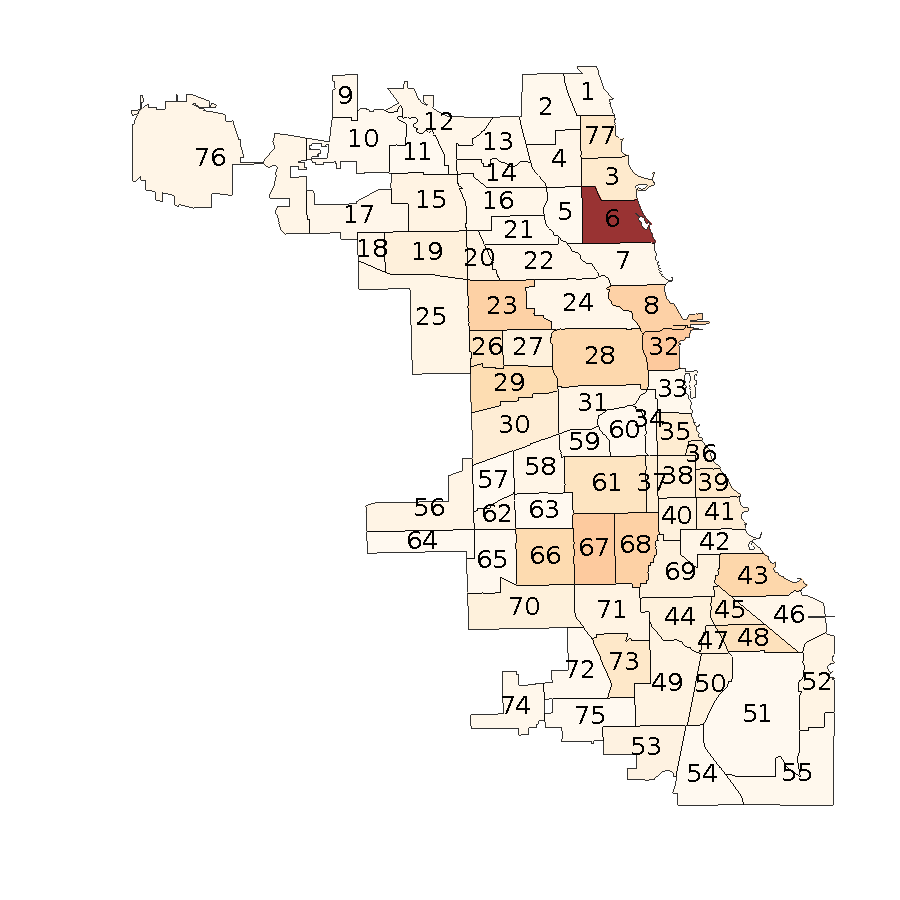
\includegraphics[width=0.4\linewidth]{fig/error_heatmap.pdf}
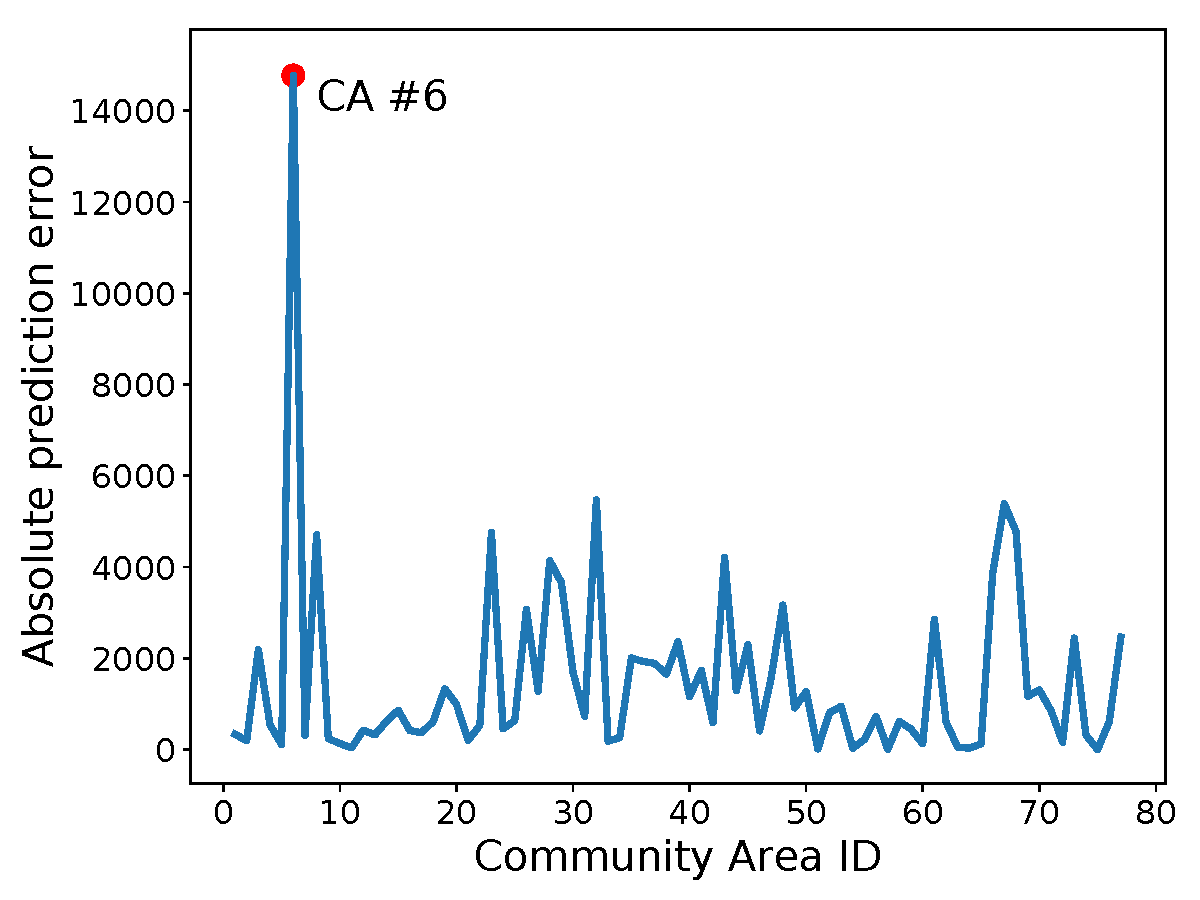
\includegraphics[width=0.5\linewidth]{fig/ca-abs-errors.pdf}
\caption{Crime prediction error at community level in Chicago. The community area \#6 is an outlier with a large error.}
\label{fig:intro}
\end{figure}

\begin{figure}
\centering
\subfigure[Census tracts of community \#6.]{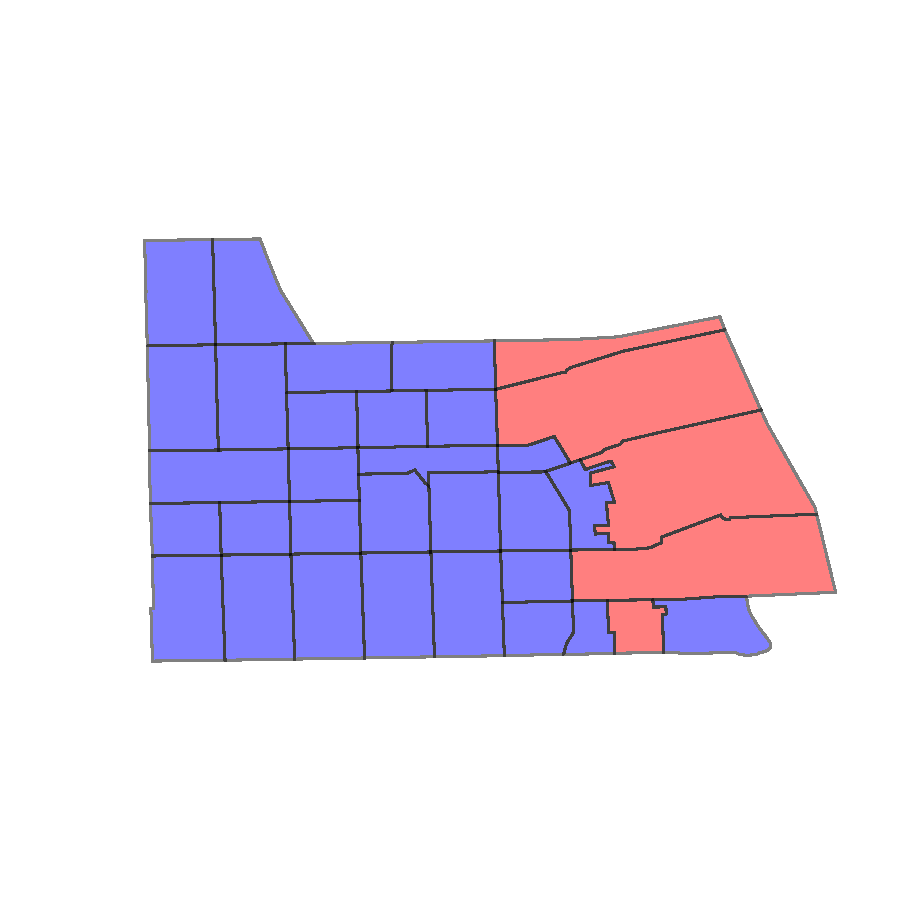
\includegraphics[width=0.5\linewidth]{fig/tracts_within_CA.pdf}}
\subfigure[Tract similarity.]{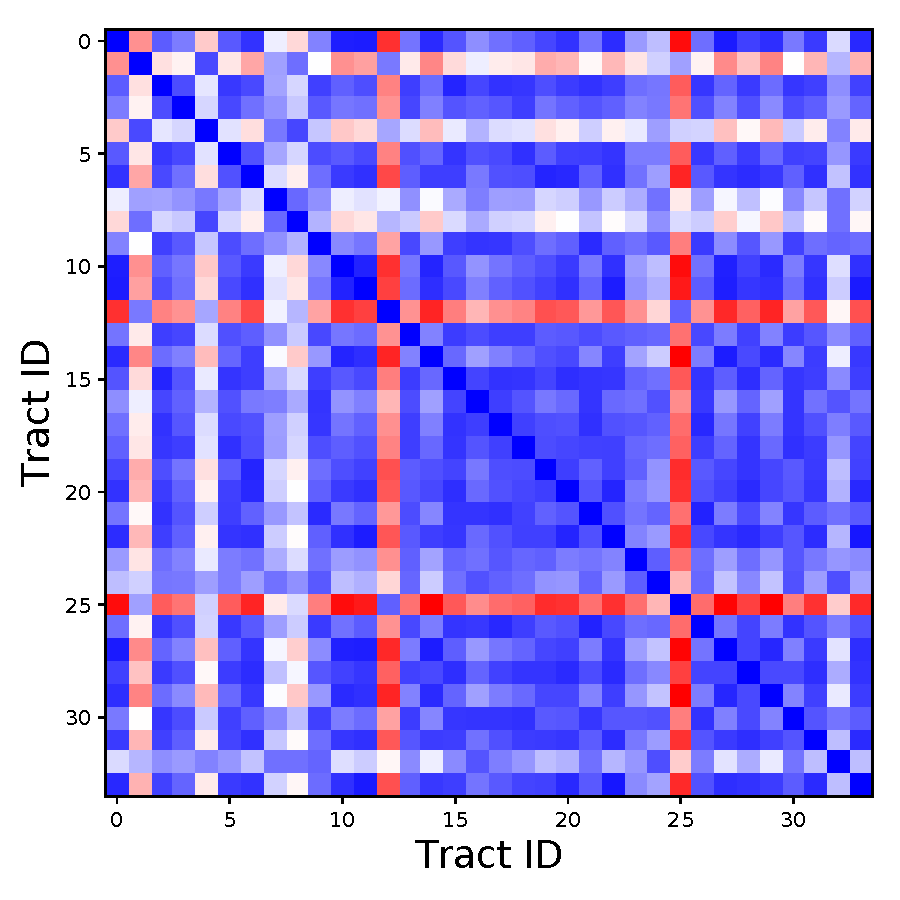
\includegraphics[width=0.45\linewidth]{fig/tract_sim_matrix.pdf}}
\caption{Explaining the outlying community area \#6 in Figure~\ref{fig:intro}. (a) Visualization of the 34 tracts in community \#6. (b) The pair-wise similarity of 34 tracts in terms of demographic features. It is clear that five tracts (in red color) on the east side are different from the other blue tracts.}
\label{fig:intro-explain}
\end{figure}

\begin{example}
Following previous work~\cite{wang2016crime}, we construct a negative binomial model to predict crime count using demographic features by treating each community area as a data sample. Figure~\ref{fig:intro} plots the crime prediction error for each community area of Chicago. Community area \#6 (i.e., Lake View area) shows an abnormally high error. In order to explain this outlier, we further investigate the internal structure of this area. Community \#6 consists of 34 census tracts as shown in Figure~\ref{fig:intro-explain}(a).  In Figure~\ref{fig:intro-explain}(b), we visualize  pair-wise Euclidean distance between tracts based on demographic features. There are five tracts that are different from the other tracts in the demographic feature space, and they are all located on the east side of community \#6. These five tracts, when mixed with other tracts in this community, lead to inferior performance of crime count prediction in that area. 
\end{example}

% problem definition
The observation above motivates us to learn a better region definition for crime study. In this chapter, we propose a new problem of \emph{task-specific region partitioning}. Given spatial variables and a selected model  (e.g., linear regression), we aim to partition the city into regions such that the model trained by taking regions as data samples achieves the optimal results.

% literature
%two lines of literature: (1) clustering, no target; (2) partition tracts into regions, and build a model for each region.
To the best of our knowledge, task-specific region partitioning is a new problem that has not been studied before. While there exist many methods for spatial clustering~\cite{miller2009geographic}, most of them group the locations based on the similarity of their spatial properties and do not have a target variable to predict. Another similar problem is to partition the locations into $k$ regions and fit a model for each region. Such a problem definition has a different purpose with the goal of showing that the correlations between features and target vary over the space (e.g., in some area, disadvantage index  correlates with crime; while in some other areas, it does not). In our problem definition, we aim to fit one model for the whole city hoping to get a generalized interpretation (e.g., disadvantage index significantly correlates with crime count in Chicago). Such a problem definition is a frequently adopted form in the criminology literature~\cite{graif2014urban}.

% challenge & proposed solution
Task-specific city region partitioning is a challenging problem. The key challenge lies in that the region properties (both features and target variable) and the model coefficients change simultaneously when we change the region partition. We prove that this is an NP-hard problem. In our proposed solution, we employ the Markov Chain Monte Carlo (MCMC) method. We start from a pre-defined region partition (e.g., community areas), and generate a new partition sample by flipping the membership of a smaller area (e.g., a tract). Two variants of MCMC methods are proposed to solve this problem. First, a naive MCMC method generates the next partition sample by randomly flipping a tract. Second, a heuristic-based MCMC method generates the next sample by flipping one tract randomly selected from the community areas with the highest error. Finally, we employ reinforcement learning to automatically learn how to generate the next sample that is more likely to improve the prediction performance.


% Experiments results
We evaluate our method on two real datasets, i.e. crime count and real estimate price. The learned region partitions are shown to consistently outperform the administrative boundaries and spatial clustering method. For example, our methods, on average, outperform the administrative boundary by $56\%$ in a crime prediction task. We also observe that the heuristic-based MCMC converges faster than the naive MCMC, while the reinforcement learning uses the least iterations to converge.

% Key contributions
To summarize, the key contributions of this chapter are:
\begin{itemize}[leftmargin=*]
\item We propose a novel problem on task-specific region partitioning. This problem is motivated by real-world urban studies, including our own previous work on crime prediction~\cite{wang2016crime}.
\item We prove the problem is NP-hard and we study different MCMC and reinforcement learning sampling techniques to solve the problem. 
\item We validate our method through extensive experiments on two real datasets.
\end{itemize}


% chapter organizations
The rest of this chapter is organized as follows. The formal definition of our problem is given in Section~\ref{ch4-sec:problem}, and our method is described in Section~\ref{ch4-sec:method}. Section~\ref{ch4-sec:experiment} shows the evaluations on two different tasks. Section~\ref{ch4-sec:related-work} summarizes related work.  Finally, we conclude in Section~\ref{ch4-sec:conclusion}.


% !TEX root = main.tex

\section{Inference Model}
\label{sec:model}


\subsection{Linear Regression}


The most straightforward prediction model is linear regression. This model assumes that the error term for $y_i$ follows a Gaussian distribution $\epsilon_i \sim \mathcal{N}(0, \sigma^2)$.


Equation~(\ref{eq:lrm}) gives the linear regression formulation of our problem:
\begin{equation}
\label{eq:lrm}
\y =  \alpha^T X^N + \beta^f W^f \y + \beta^g W^g \y + \epsilon.
\end{equation}
$X^N \in R^{d_N \times n}$ is the nodal feature matrix where column $i$ is the nodal feature vector of region $i$, $d_N$ is the dimension of nodal features, and $n$ is the number of regions. Both demographic features and POI distribution features are included in $X^N$ as nodal features. $W^f \in \R^{n \times n}$ is the flow matrix of taxi flow, and $W^g \in \R^{n \times n}$ is the spatial matrix representing the geographical adjacency. In addition, $\alpha \in \R^{d_N}$ and $\beta^f, \beta^g \in \R$ are the coefficients for corresponding features. Note that $\epsilon \in \R^n$ is the only stochastic variable on the right-hand side; all other terms are fixed observation values. Therefore, we incorporate all the fixed observations into one term $X \in \R^{(d_N + 2)\times n}$, and we get the standard regression problem:
\[
\y= \w^T X + \epsilon,
\]
where $\w = [\alpha^T, \beta^f, \beta^g]^T$ is the concatenation of all coefficients.


\subsection{Negative Binomial Regression}


In our problem, we aim to infer the crime rate, which is guaranteed to be a non-negative integer. However, linear regression does not ensure this property. 
\emph{Poisson regression} is another form of regression, more appropriate for non-negative data than linear regression \cite{GMS95, Lamb92}. With shortened notation $\x_i$, which represents all features in a region, the Poisson regression model has the exponential function as link function
\begin{equation}
\label{eq:prm}
E(y_i) = e^{\w^T \x_i}.
\end{equation}
In the following, we omit the index $i$ wherever it is clear to refer to the variable of a single region.
The link function comes from the assumption that $y$ follows the Poisson distribution with mean $\lambda $. Additionally, the mean $\lambda$ is determined by observed independent variables $\x$, i.e. $\lambda = e^{\w^T \x}$. Adding all together, the joint probability of $y$ is 
\begin{equation}
P(y|\w) = \frac{e^{-e^{\w^T\x}}(e^{\w^T\x})^y}{y!}.
\end{equation}


However, Poisson regression enforces the mean and variance of dependent variable $y$ to be equal. This restriction leads to the ``over-dispersion'' issue for some real problems, that is the presence of larger variability in data set than the statistical model expected. To address this,  we use the Poisson-Gamma mixture model, which is also known as \emph{negative binomial regression}. Negative binomial regression is frequently used in crime research \cite{Osg00}.

Given that the crime rate $y$ follows Poisson distribution with mean $\lambda$, in order to allow for larger variance, $\lambda$ itself is a random variable having a Gamma distribution with shape $k$ and scale $\theta = \frac{p}{1-p}$.  The probability density function of $y$ becomes
\begin{align}
\label{eq:nbpdf}
P(y|k, p) & = \int_0^{\infty} P_{Poisson}(y|\lambda) \cdot P_{Gamma}(\lambda|k, p) d \lambda \nonumber \\
		& = \int_0^{\infty} \frac{\lambda^y}{y!} e^{-\lambda} \cdot \lambda^{k-1} \frac{e^{-\lambda(1-p)/p}}{(\frac{p}{1-p})^k \Gamma(k)} d\lambda  \nonumber \\
		 & = \frac{\Gamma(k+y)}{y! \Gamma(k)} p^y (1-p)^k.
\end{align}
This is exactly the probability density function of negative binomial distribution.


In negative binomial regression, the link function is
\begin{equation}
E(y) = e^{\w^T \x + \epsilon }.
\end{equation}
The error term $e^\epsilon$ is the mixture prior from the Gamma distribution, and we assume its mean is $1$, i.e. $E(e^\epsilon) = 1$. This setting ensures that $E(y) = e^{\w^T \x} \cdot e^\epsilon = e^{\w^T \x}$. Meanwhile, given the probability density function of negative binomial distribution in Equation~(\ref{eq:nbpdf}), the mean of negative binomial distribution is $\frac{pk}{1-p}$. Combining the theoretical mean with the link function, we have $p = \frac{e^{\w^T\x}}{e^{\w^T\x} + k}$. Therefore, the probability mass function of $y$ becomes
\begin{equation}
\label{eq:nbpdf2}
P(y| \w, k) = \frac{\Gamma(k+y)}{y! \Gamma(k)} \left(\frac{e^{\w^T\x}}{e^{\w^T\x} + k}\right)^y \left(\frac{k}{e^{\w^T\x} + k}\right)^k.
\end{equation}


The log-likelihood function of negative binomial model is given in Equation~(\ref{eq:nbpdf2-ll}), where $w$ and $\theta$ can be estimated by maximizing likelihood.
\begin{multline}
  \label{eq:nbpdf2-ll}
\mathcal{L}(\w, k; \y, X) =	\sum_{i=1}^n \Bigg\{y_i \ln\left( \frac{e^{\w^T \x_i}}{e^{\w^T \x_i} + k}\right) + k \ln\left(\frac{k}{e^{\w^T \x_i} +k}\right) \\
	+ \ln \Gamma(y_i + k ) - \ln \Gamma(y_i + 1) - \ln \Gamma( k) \Bigg\}.
\end{multline}



\subsection{Non-Stationary Model}


The two regression models described above assume the statistical correlations between crime rate and observed features are constant over space, because they learn one set of parameters for all community areas. In the real world, it is very likely that some statistical correlations between crime rate and observed features are not stationary over space. In this section we propose to apply a non-stationary model, called geographically weighted regression (GWR)~\cite{FBC03}, to capture the different crime correlations at different places.

Formally, a global spatial regression model such as the aforementioned two models has the following form
\begin{equation}
y = f(\x, \w),
\end{equation}
where $\w$ is the parameter of the regression function $f$. Given a set of data points $\{y_i, \x_i\}_{i=1}^n$ sampled at locations $l_1, \cdots, l_n$, the maximum likelihood estimation of parameter $\w$ is given by 
\begin{equation}
\w^* = \argmax_{\w} \sum_{i=1}^n \mathcal{L} (  y_i, f(\x_i, \w) ).
\end{equation}
This global model is stationary, because the weights used for predictions are the same at all locations, when we fit the model to find the optimal parameter.

Instead, the GWR learns a \emph{local} regression function $f$ with parameter $\w_i$ at each location of interest $l_i$: 
\begin{equation}
\label{eq:gwrs}
y = f(\x, \w_i),  \quad \forall l_i \in \{l_1, l_2, \cdots, l_n\},
\end{equation}
where $l_i$ is usually a geospatial coordinate in the two dimensional space. In order to train a lot of local models, we need a larger number of samples at each location $l_i$, which are usually not available. To address this issue, GWR uses the spatially nearby samples and gives each sample a weight according to the distance between sample point and target location $l_i$. The objective for the local model at location $l_i$ is 
\begin{equation}
\label{eq:gwr-general}
\w_i^* = \arg\min_{\w_i} \sum_{j=1}^n  \gamma_{ij} \mathcal{L} \left(y_j, f(\x_j, \w_i) \right),
\end{equation}
where $\gamma_{ij}$ is the spatial kernel to weight the neighboring data point at location $l_j$ for regression model at location $l_i$.


\textbf{Choice of spatial kernel $\gamma$}. There are several spatial kernels we can choose from. The most straightforward solution is to exclude samples that are further away from target location. Namely,
\begin{equation}
\gamma_{ij} = \left\{ \begin{array}{ll}  1 & \text{if $d_{ij} < \tau$} \\  0 & \text{otherwise,} \end{array} \right.
\end{equation}
where $d_{ij}$ is the distance between $l_i$ and $l_j$, and $\tau$ is a distance threshold. Clearly, such a solution suffers from the discontinuity. 

A better solution is to specify the weight $\gamma$ as a continuous function of distance $d$, which is
\begin{equation}
\label{eq:gwr-gkn}
\gamma_{ij} = \exp\left( -\frac{d_{ij}^2}{2h^2} \right),
\end{equation} 
where $h$ is referred to as the bandwidth of the Gaussian kernel. Intuitively, when the samples are dense near the target location $l_t$, the $h$ can be set smaller, so that we give lower weights to those samples far away. On the other hand, if the samples are sparse, $h$ should be set larger, so that we consider those further away samples as well to train our model. When $h$ is set to infinity, the GWR becomes a global model, since all samples have equal weight $1$. 


One issue with the Gaussian kernel in Equation~(\ref{eq:gwr-gkn}) is that when the samples are dense, it over-smooths local models by considering too many samples at each location. A popular alternative kernel utilizes the bi-square function,
\begin{equation}
\gamma_{ij} = \left\{ \begin{array}{ll}  \left( 1 - \frac{d_{ij}^2}{\tau^2}\right)^2 & \text{if $d_{ij} < \tau$} \\  0 & \text{otherwise.} \end{array} \right.
\end{equation}
The bi-square kernel functions provides continuous weight for samples up to distance $\tau$. In our problem, since we do not have too many samples available, therefore we use the Gaussian kernel, and in experiment we will show the bandwidth tuning to get the best results.


\textbf{Applying GWR on existing methods}. The GWR is more like a framework rather than a method, which can be applied to many existing regression methods. The classic GWR is applied to linear regression model resulting in the following objective for location $l_i$  
\begin{equation}
\w_i^* = \arg\min_{w_i} \sum_{j=1}^n \gamma_{ij} (y_j - \w_i^T \x_j)^2.
\end{equation}
% We can use the commonly used least square estimation to find the best $w_i$, because the $\gamma_k$ can be calculated in advance.


Similarly, the GWR framework can be employed with the negative binomial regression model, and we call this \emph{geographically weighted negative binomial regression} (GWNBR). Here, the objective for model at location $l_i$ is to optimize the weighted log-likelihood function:
\begin{multline}
\label{eq:finalObj}
\mathcal{L}(\w_i, k_i; \y, X) = \\
	\sum_{j=1}^n \gamma_{ij} \Bigg\{y_j \ln\left( \frac{e^{\w_i^T \x_j}}{e^{\w_i^T \x_j} + k_i}\right) + k_i \ln\left(\frac{k_i}{e^{\w_i^T \x_j} +k_i}\right) \\
	+ \ln \Gamma(y_j + k_i ) - \ln \Gamma(y_j + 1) - \ln \Gamma( k_i) \Bigg\}.
\end{multline}


\subsection{Optimization}

The objective in Equation~(\ref{eq:finalObj}) can be solved using a block coordinate gradient descent method, by alternatively solving $\w_i$ and $k_i$. Details for solving each step are given below.\\
\textbf{Fix $k_i$, solve $\w_i$:}\\
When $k_i$ is fixed, the objective function can be simplified as follows:
\begin{multline}
	\min_{\w_i}
	-\sum_{j=1}^n \gamma_{ij} \Bigg\{y_j \ln\left( \frac{e^{\w_i^T \x_j}}{e^{\w_i^T \x_j} + k_i}\right) + k_i \ln\left(\frac{k_i}{e^{\w_i^T \x_j} +k_i}\right) \}.
\end{multline}
The gradient is:
\begin{equation}
	\frac{\partial \mathcal{L}}{\partial \w_i}=\sum_{i=1}^{n}\gamma_{ij}\{y_i\frac{\x_je^{\w_i^T\x_j}}{e^{\w_i^T\x_j}}-\frac{(y_i+k_i)\x_je^{\w_i^T\x_j}}{e^{\w_i^T\x_j}+k_i}\}.
\end{equation}
Then,
\begin{equation}
\w_i^t=\w_i^{t-1}+\alpha\frac{\partial \mathcal{L}}{\partial \w_i^{t-1}}.
\end{equation}
\textbf{Fix $\w_i$, solve $k_i$:}\\
When $\w_i$ is fixed, the objective function becomes:
\begin{multline}
\min_{k_i} = \\
-\sum_{j=1}^n \gamma_{ij} \Bigg\{y_j \ln\left( \frac{e^{\w_i^T \x_j}}{e^{\w_i^T \x_j} + k_i}\right) + k_i \ln\left(\frac{k_i}{e^{\w_i^T \x_j} +k_i}\right) \\
+ \ln \Gamma(y_j + k_i ) - \ln \Gamma( k_i) \Bigg\}.
\end{multline}
The gradient is:
\begin{multline}
	\frac{\partial \mathcal{L}}{\partial k_i}=\sum_{i=1}^{n}\gamma_{ij}\{\frac{y_i}{e^{\w_i^T\x_j}+k_i}+\ln(\frac{k_i}{e^{\w_i^T\x_j}+k_i})\\-\frac{k_i}{e^{\w_i^T\x_j}+k_i}+1+\psi(y_j+k_i)-\psi(k_i)+y_i\},
\end{multline}
where $\psi(x)=\frac{\Gamma'(x)}{\Gamma(x)}$ is digamma function. Then,
\begin{equation}
k_i^t=k_i^{t-1}+\alpha\frac{\partial \mathcal{L}}{\partial k_i^{t-1}}.
\end{equation}

% !TEX root = main-crime.tex

\section{Feature Extraction}
\label{ch2-sec:feature}

%As discussed in Section~\ref{sec:overview}, there are three types of features used in inference model. 
In this section, we will discuss the details of features used in our method. The two types of new features we use are extracted from Point-Of-Interest data and taxi flow data. Below we describe the datasets used to construct features and the characteristics of these features.

\begin{figure*}[t]
\centering
\subfigure[Total population]{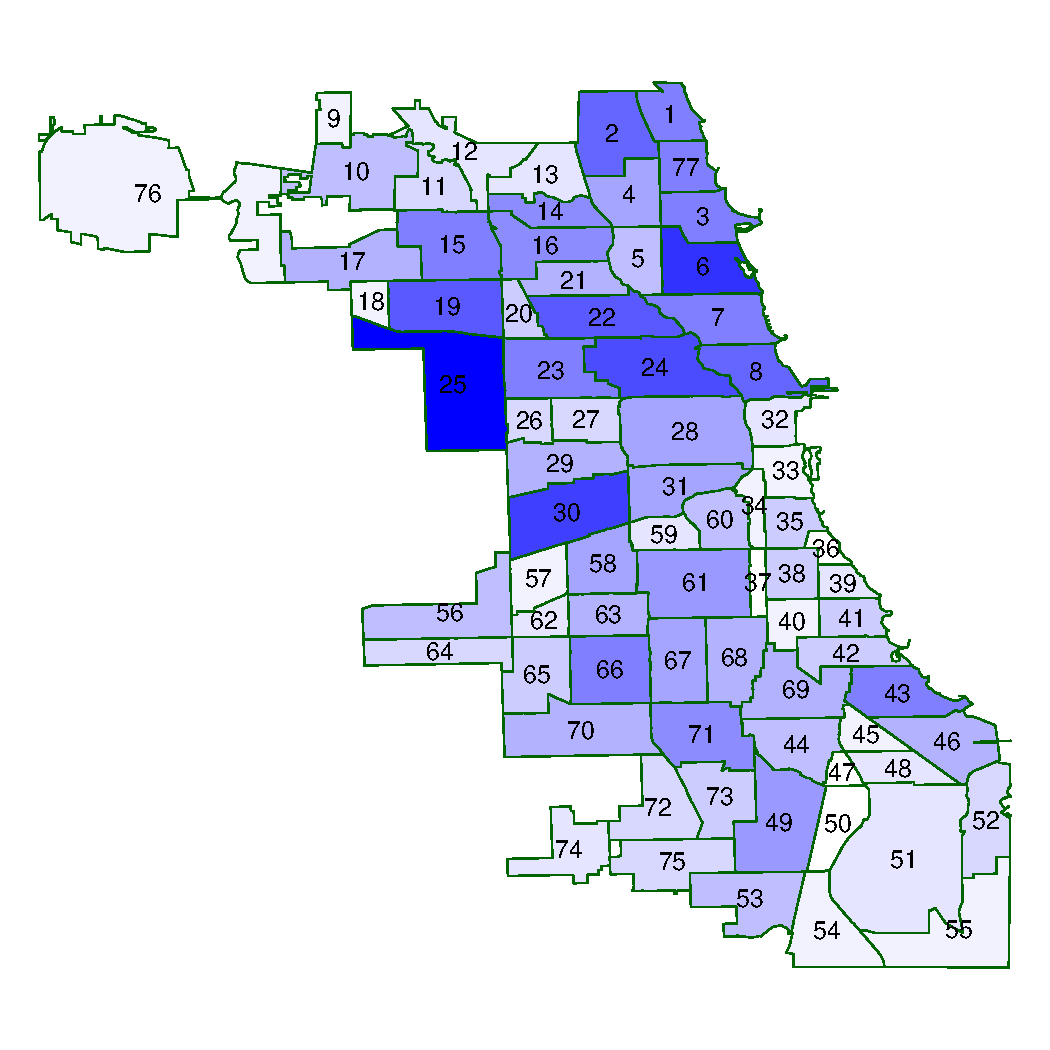
\includegraphics[width=0.45\textwidth]{fig/demo-f1.pdf}}
%\subfigure[Population density]{\includegraphics[width=0.22\textwidth]{fig/demo-f2.pdf}}
\subfigure[Poverty index]{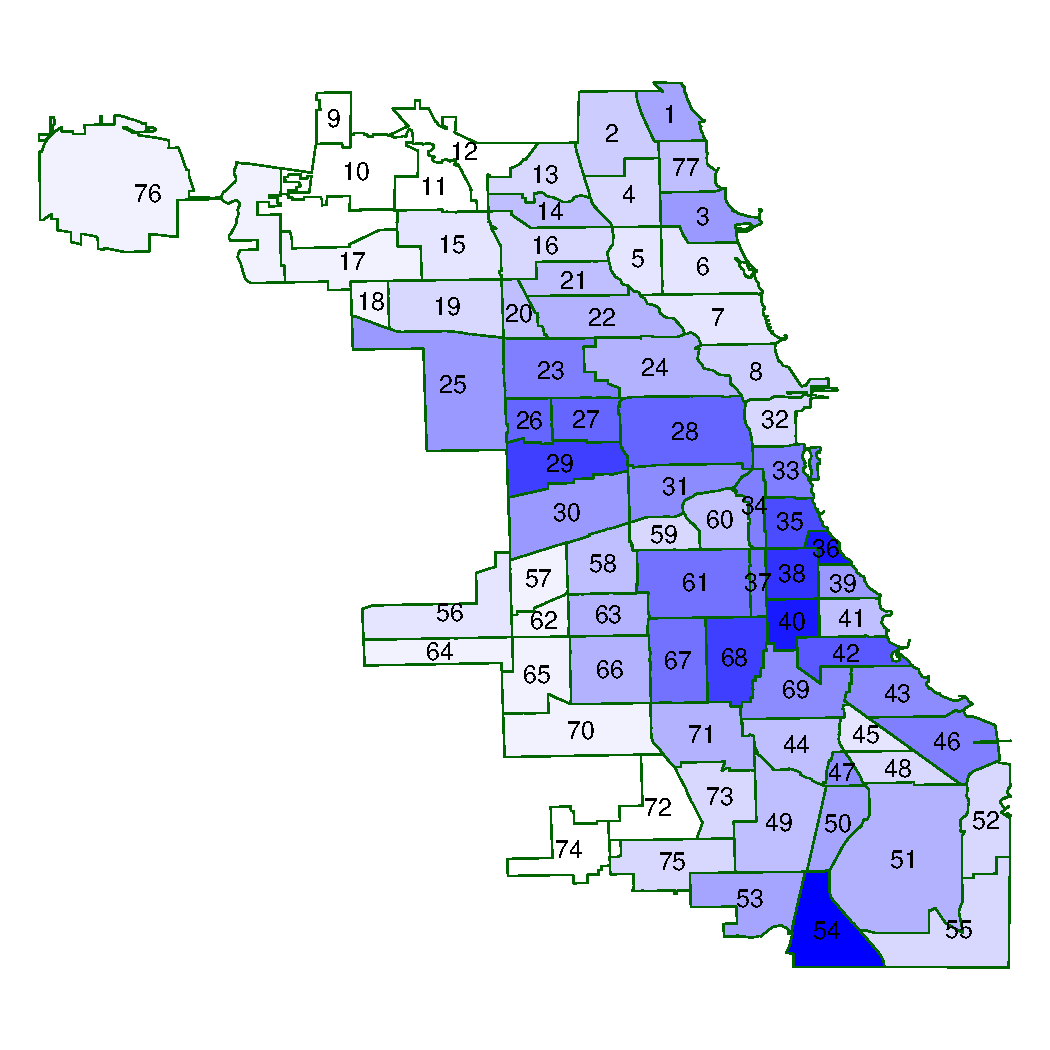
\includegraphics[width=0.45\textwidth]{fig/demo-f3.pdf}}
\subfigure[Disadvantage index]{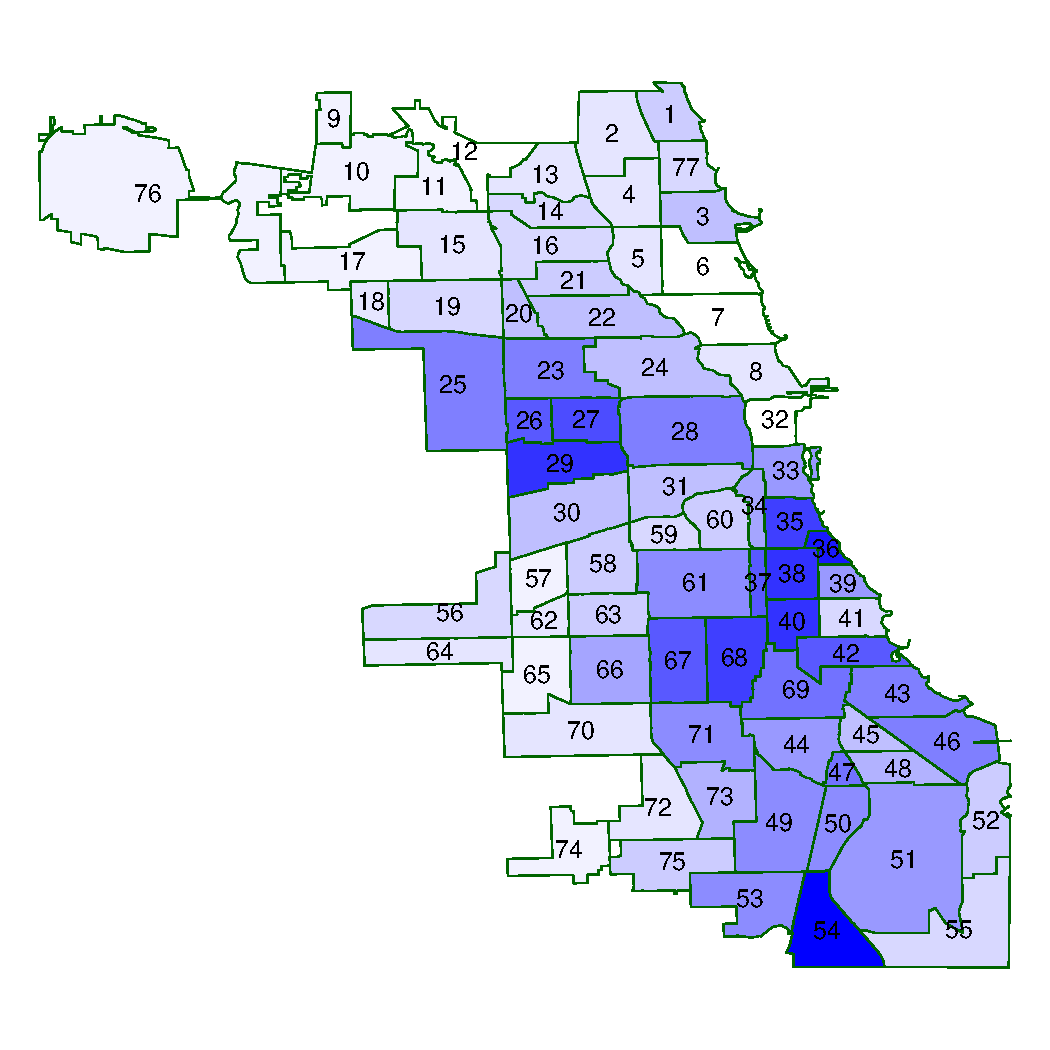
\includegraphics[width=0.45\textwidth]{fig/demo-f4.pdf}}
%\subfigure[Residential stability]{\includegraphics[width=0.22\textwidth]{fig/demo-f5.pdf}}
\subfigure[Ethnic diversity]{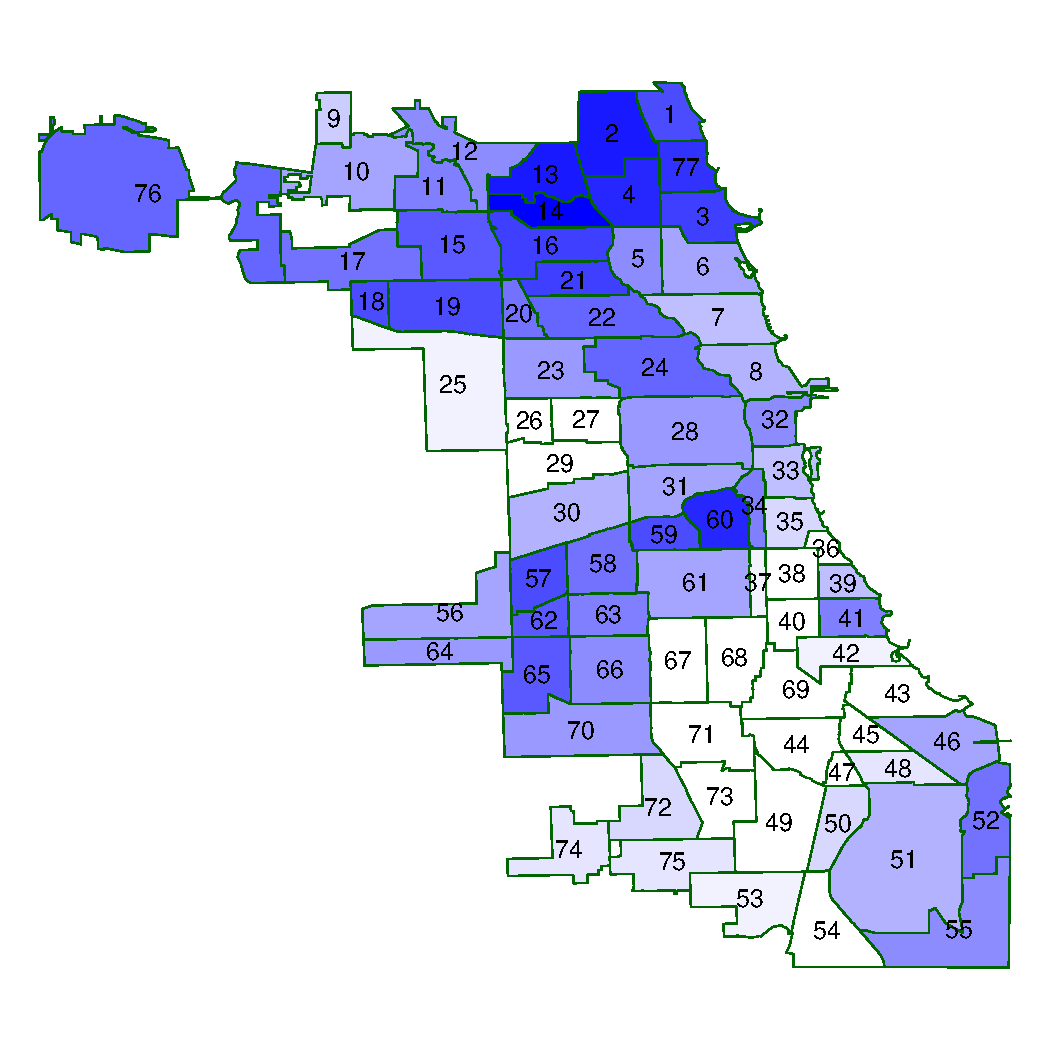
\includegraphics[width=0.45\textwidth]{fig/demo-f6.pdf}}
%\subfigure[Percentage black]{\includegraphics[width=0.22\textwidth]{fig/demo-f7.pdf}}
%\subfigure[Percentage Hispanic]{\includegraphics[width=0.2\textwidth]{fig/demo-f8.pdf}}
%\subfigure[\textred{Percentage white}]{\includegraphics[width=0.2\textwidth]{fig/demo-f8.pdf}}
\caption{(a)-(d) Demographics in Chicago by community areas. Darker colors indicate higher values. Each demographic feature is normalized into $[0,1]$.}
\label{fig:demo-f}
\end{figure*}





\subsection{Nodal Feature: Demographics}

Socioeconomic and demographic features of neighborhoods have been
widely used to predict crime~\cite{Bogo14, HsPu93, WoMe12, SaHi07}. Previous studies have shown that crime rate correlates with certain demographics. For example, \cite{Jac61, GrSa09} suggests that population diversity leads to less crime in certain neighborhoods. 
In our study, we include demographic information from the US Census Bureau's Decennial Census ~\cite{census-data}.   Using 2010 census information would overlap with the time in which crime is measured. Instead, we use year 2000 demographic data because we are interested in predictors that precede temporally the period in which crime rates are evaluated. The demographics include the following features:

\textsf{total population, population density, poverty, disadvantage index, residential stability, ethnic diversity, race distribution}.


The poverty index measures the proportion of community area residents
with income below the poverty level. The disadvantage index is
a composite scale based on prior work \cite{SRE97}, a function of 
poverty, unemployment rate, proportions of families with public
assistance income, and proportion of female headed households. 
 The residential stability measures home ownership and proportion of
residents who lived in the neighborhood for more than one year. Racial
and ethnic diversity is an index of heterogeneity~\cite{GrSa09} based on six
population groups, including: Hispanics, non-Hispanic Blacks, Whites,
Asians, Pacific Islanders and others.


Figure~\ref{fig:demo-f} visualizes the crime rate and demographics features in Chicago by community areas. Comparing with Figure~\ref{fig:crime-ca}, it is clear that the crime rate and poverty index and disadvantage index are consistent,  the ethnic diversity shows an inverse correlation, and the total population has little correlation with crime.



Table~\ref{tb:demo} shows the Pearson correlation coefficient between various demographics features and the crime rate at community area level. The corresponding p-value is also calculated and shown in the table to indicate the significance of the correlation coefficient.  There  are in total $77$  community areas in Chicago. Table~\ref{tb:demo} shows such correlation with several most correlated features. We can see that the poverty index and disadvantage index positively and strongly correlate with crime, while the ethnic diversity negatively correlates with crime. Other features such as total population, population density, and residential stability  have weaker correlations. One counter-intuitive observation is that the total population has a weak and negative correlation with crime. The reason is that we use crime rate in each community area, which is already normalized by the population, and therefore the total population and population density have less impact. 


\begin{table}[h]
\vspace{-5mm}
\centering
\caption{Pearson correlation between demographic features  and crime rate (\textbf{*} indicates significant correlations with p-value less than $5\%$). }
\begin{tabular}{|c||c|c|}
\hline
Feature & Correlation & p-value \\ \hline \hline
Total Population & -0.1269 &  0.2716 \\ \hline
Population Density & -0.1972  & 0.0855 \\ \hline
Poverty Index & \textbf{0.5573*} & 1.403e-07 \\ \hline
Disadvantage Index & \textbf{0.5959*} & 1.082e-08 \\ \hline
Residential Stability  & -0.0453 &  0.6965 \\ \hline
Ethnic Diversity & \textbf{-0.5545*} &  1.678e-07 \\ \hline
Percentage of Black & \textbf{0.6696*} &  2.779e-11 \\ \hline
Percentage of Hispanic  & \textbf{-0.3820*} &  0.0006 \\ \hline
\end{tabular}
\label{tb:demo}

\end{table}

\nop{
\begin{table}[h]
\centering
\caption{Demographic feature description and correlation with crime.}
\vspace{-5mm}
\begin{tabular}{|l|l|r|r|}
\hline
Abbr. & Description & Pearson & p-value \\ \hline
TP & total population & -0.1269 &  0.2716 \\ \hline
PD & population density & -0.1972  & 0.0855 \\ \hline
PI & poverty index & 0.5573 & 1.403e-07 \\ \hline
DI & disadvantage index & 0.5959 & 1.082e-08 \\ \hline
RS & residential stability  & -0.0453 &  0.6965 \\ \hline
ED & ethnic diversity & -0.5545 &  1.678e-07 \\ \hline
PB & percentage of Black & 0.6696 &  2.779e-11 \\ \hline
PH & percentage of Hispanic  & -0.3820 &  0.0006 \\ \hline
\end{tabular}
\label{tb:demo}
\end{table}
}


\subsection{Nodal Feature: Point-of-Interest (POI)}

While demographics are traditional census data, POI is a type of  modern data that provide fine-grained information about locations. We collect POI from FourSquare~\cite{poi-data}. POI data from FourSquare provide the venue information including venue name, category, number of check-ins, and number of unique visitors. We mainly use the major category information because categories can characterize the neighborhood functions. There are 10 major categories defined by FourSquare:

\textsf{food, residence, travel, arts \& entertainment, outdoors \& recreation, college \& education, nightlife, professional, shops, and event.}


\begin{figure}[tb]
\centering
%\subfigure[Food]{\includegraphics[width=0.2\textwidth]{fig/poi-dist1.pdf}}
\subfigure[Nightlife]{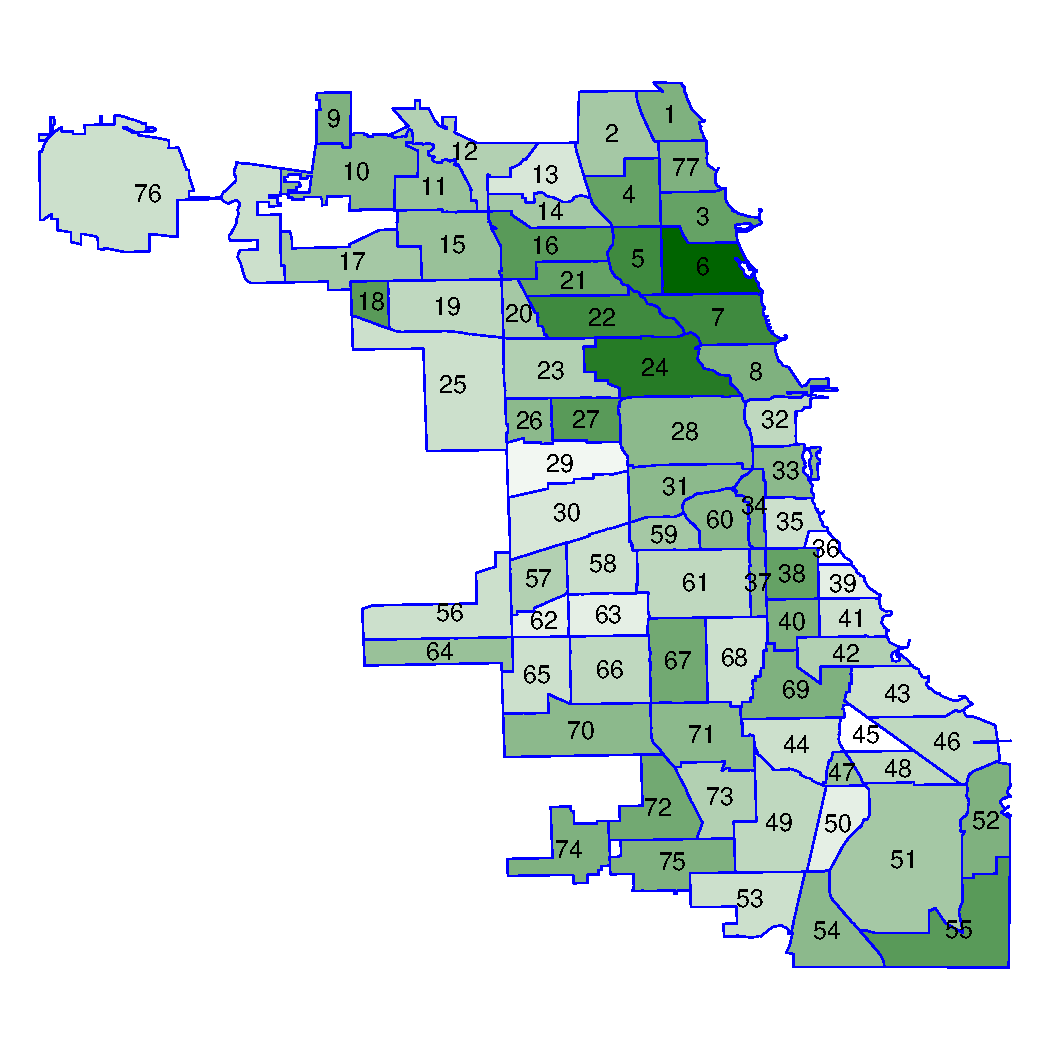
\includegraphics[width=0.45\textwidth]{fig/poi-dist7.pdf}}
%\subfigure[Travel]{\includegraphics[width=0.2\textwidth]{fig/poi-dist3.pdf}}
\subfigure[Professional]{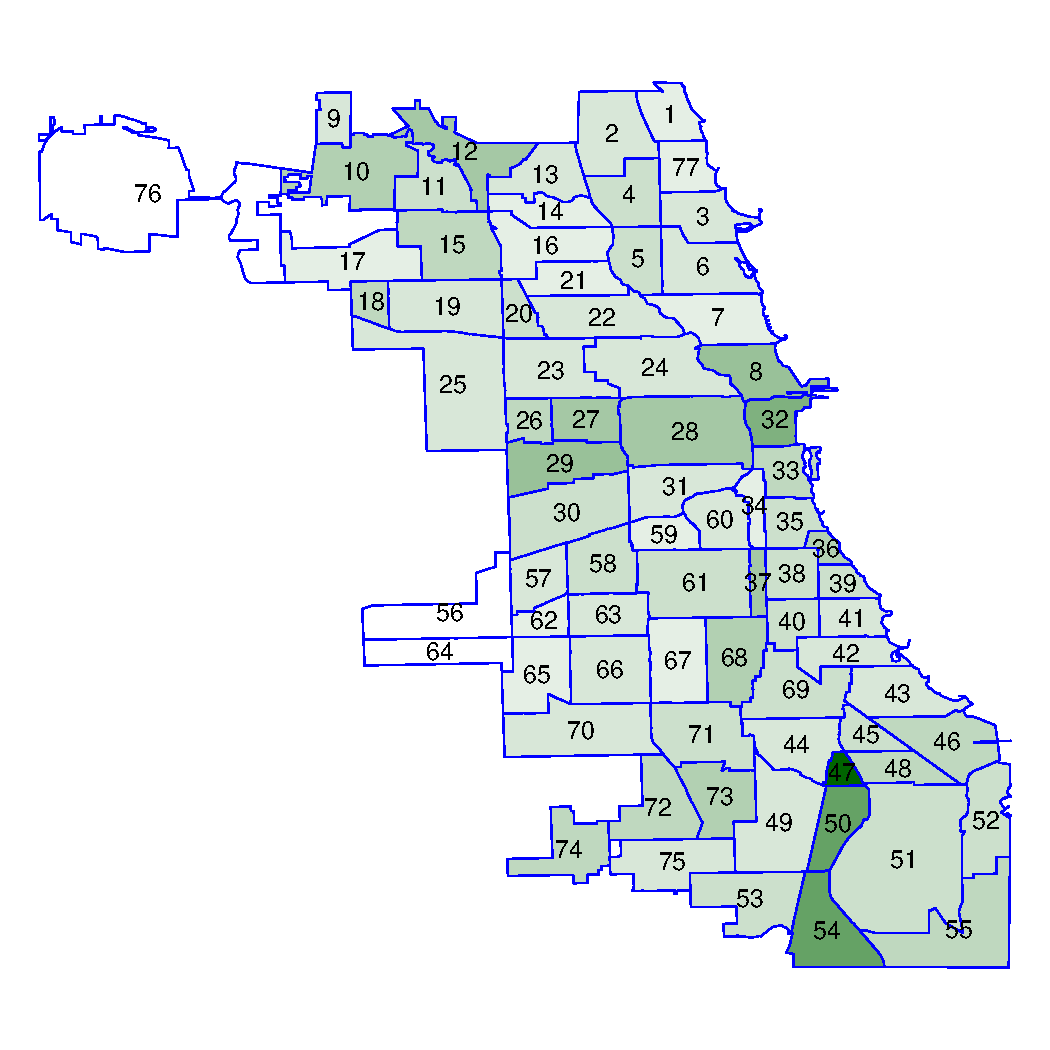
\includegraphics[width=0.45\textwidth]{fig/poi-dist8.pdf}}
%\subfigure[Shops]{\includegraphics[width=0.2\textwidth]{fig/poi-dist9.pdf}}
\caption{POI ratio per neighborhood. The saturation of color is proportional to the ratio value. The ``professional'' category distribution is more consistent with the crime distribution, and therefore it is the most correlated with crime. Meanwhile, the ``nightlife'' category is negatively correlated with Chicago crime. The POI ratios are independently normalized for different POI categories.}
\label{fig:poi-coef}
\end{figure}

In total, we have crawled \num{112000}  POIs from FourSquare for Chicago. Most of these POIs are in the downtown area of Chicago. For the purpose of visualization, we normalize the POIs count per category by the total POI count in a neighborhood and plot two selected categories, i.e. nightlife and professional, in Figure~\ref{fig:poi-coef}.  The darker colored neighborhoods in Figure~\ref{fig:poi-coef} are the ones with a higher proportion of residence POIs.



\begin{table}[h]
\centering
\caption{Pearson correlation between POI category and crime rate (\textbf{*} indicates significant correlations with p-value less than $5\%$).}
\vspace{2mm}

\label{tb:poi-corr}
\begin{tabular}{|c ||c|c|}
\hline
POI category & Correlation & p-value \\ \hline \hline
Food & -0.1543 &  0.1803 \\ \hline
Residence &  -0.0610 &  0.5984 \\ \hline
Travel & -0.0017 &  0.9883 \\ \hline
Arts \& Entertainment & -0.0049 &  0.9661 \\ \hline
Outdoors \& Recreation &  0.0668 &  0.5637 \\ \hline
College \& Education & -0.0078 &  0.9473 \\ \hline
Nightlife &  -0.1553 &  0.1775 \\ \hline
Professional & \textbf{0.3221*} &  0.0043 \\ \hline
Shops & -0.1676 &  0.1450 \\ \hline
Event & 0.2196 &  0.0549  \\ \hline
\end{tabular}
\end{table}



In Table~\ref{tb:poi-corr} we show the Pearson correlation between POI category and crime rate. The category ``professional''  is most significantly correlated with the crime rate. Under the professional POI category, there are some venues with a large population concentration, such as transportation center, convention center, community center, and coworking space. In those venues, the  population volume is high and residential stability is low, therefore the professional POI counts positively correlates with crime rate.  One counter-intuitive observation is that ``nightlife'' category is not positively correlated with crime ($-0.1553$). This can be seen in Figure~\ref{fig:poi-coef}(a). The majority of nightlife venues in Chicago are located in the northern area, while most crime incidents occur in the downtown area.



\subsection{Edge: Geographical Influence}

Together with the US census demographics data, we also collected the boundary shape files of Chicago, which are used to calculate the geographical influence feature.
Previous studies have also shown that the crime rate at one location is highly correlated with nearby locations~\cite{GSGL01, Bur88}. Such geographical influence is also frequently used in the literature~\cite{ACC00, MoSa97}. It is calculated as:
\begin{equation}
\vec{F^g} = W^g \cdot \vec{Y},
\label{eq:spatial}
\end{equation}
where $W^g$ is the spatial weight matrix. If region $i$ and $j$ are not geospatially adjacent, $w_{ij}^g = 0$; otherwise, $w_{ij}^g \propto distance(i,j)^{-1}$.

\begin{figure}[t!]
\centering
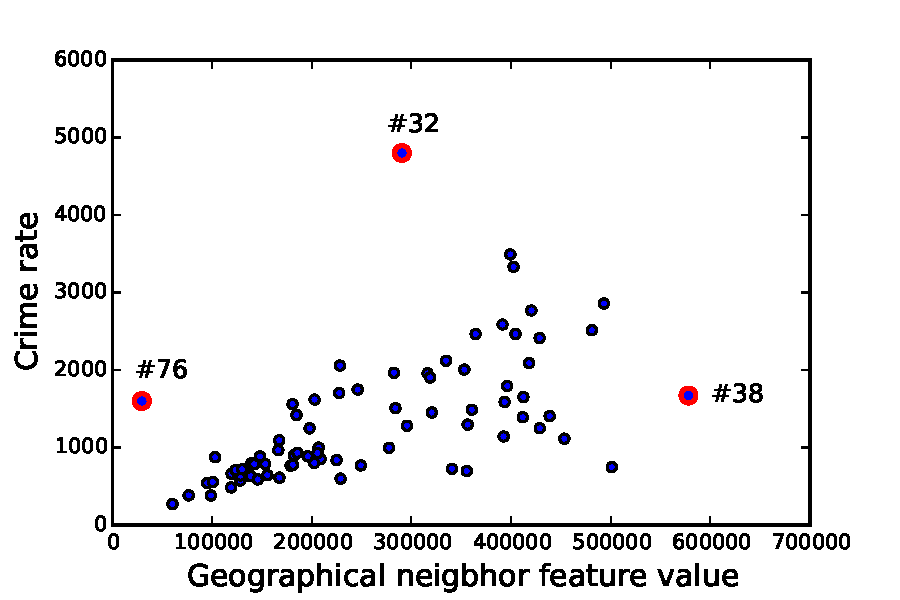
\includegraphics[width=0.8\textwidth]{fig/spatial-crime-rate.pdf}
\caption{The correlation between geographical influence feature  and crime rate. In the plot we marked out three outliers and their corresponding community area ID.}
\label{fig:spatial}
\end{figure}

In Figure~\ref{fig:spatial},  we plot crime rate with respect to geographical influence calculated in Eq.~\ref{eq:spatial}. We observe an obvious positive correlation, which means if nearby neighborhoods have a high crime rate, the focal neighborhood is more likely to have a high crime rate. We also do observe a few outliers in Figure~\ref{fig:spatial}. These neighborhoods show different crime rate in their nearby neighborhoods compared to their own. For example, as we can also see in Figure~\ref{fig:crime-ca}, community area \#38 locates in an area where the the neighbors have high crime rates but its crime rate is relatively low; in contrast, neighborhood \#32 has a high crime rate even though its neighbors have relatively low crime. The community area \#76 home of the O'Hare International Airport is far from most of other community areas, however its own crime rate is relative high.



\subsection{Edge: Hyperlinks by Taxi Flow}

In our Chicago taxi dataset, there are \num{1048576} taxi trips in total from October to December in 2013. For each trip, the following information are available: pickup/dropoff time, pickup/dropoff location, operation time, and total amount paid. We requested the taxi trip records from Chicago under the Illinois Freedom of Information Act.  Figure~\ref{fig:taxi-flow} shows a visualization of the major flows at community level.

\begin{figure}[htb]
\centering
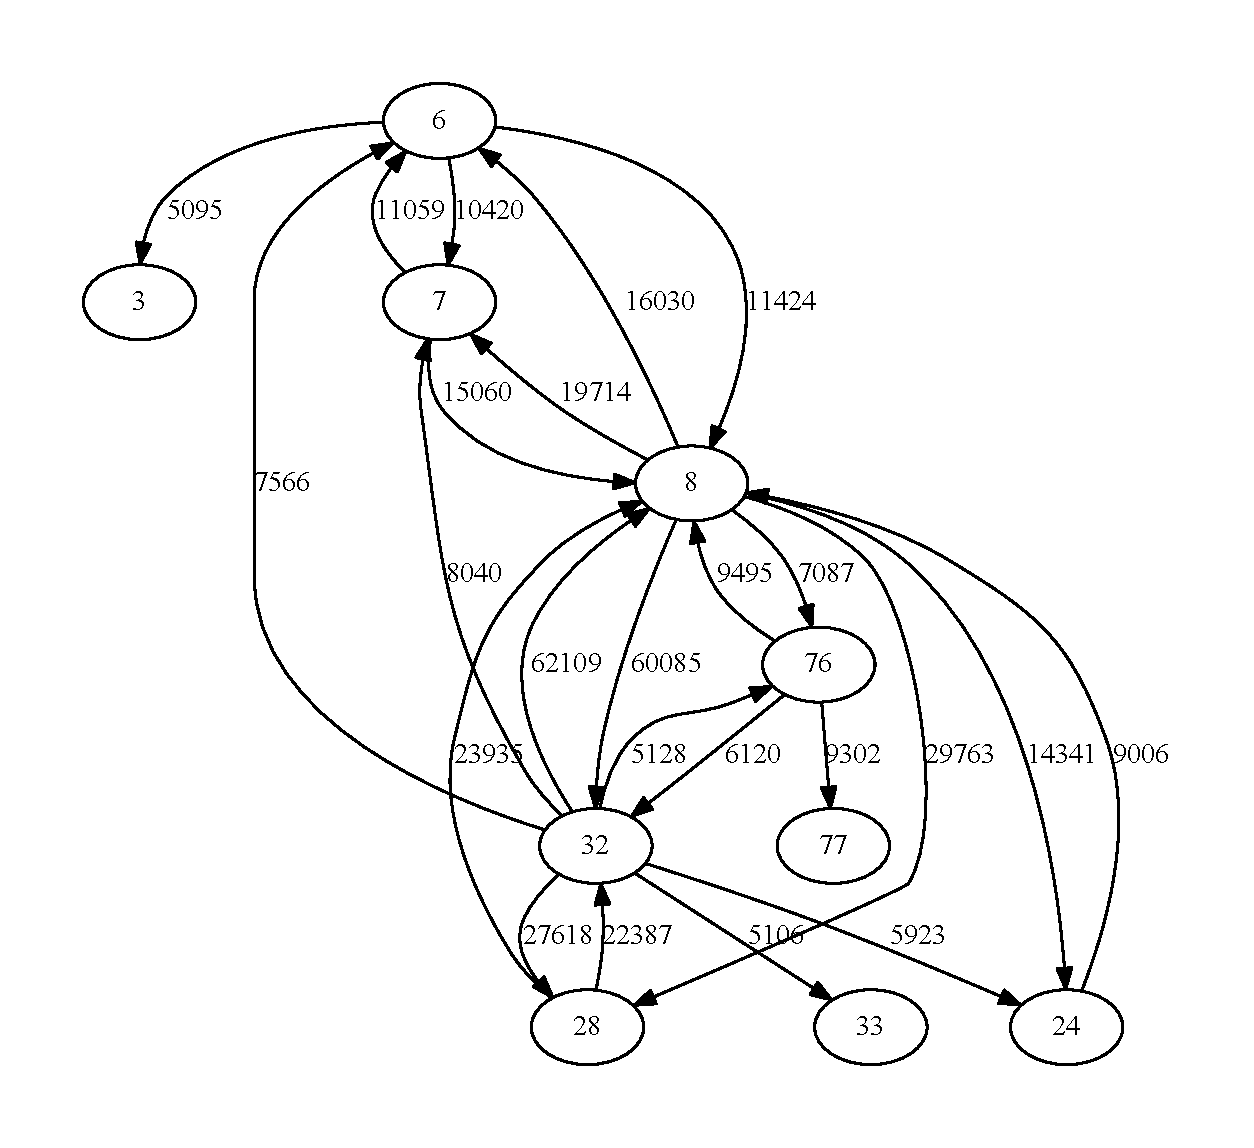
\includegraphics[width=0.7\textwidth]{fig/taxiflow.pdf}
\caption{Major taxi flows between neighborhoods. The label on the edge shows the count of taxi trips  commuting between two community areas from October to December months in 2013. We set a threshold (more than 5,000 trips) on the flow and only plot high volume flows. The label on a node is the ID of its corresponding community area. We can see that there are several hub community areas, such as \#6, \#8, \#32, which are all in the downtown areas. }
\label{fig:taxi-flow}
\end{figure}


One of our hypotheses is that the social interaction among two community areas propagates crime from one region to another.
The Chicago taxi data captures the social interactions among various community areas. To calculate this, we first map all taxi trips to community areas to get the taxi flow $w_{ij}\ \forall i,j \in \{1, 2, \cdots n\}$. Then the taxi flow lag is constructed by the product of social flow and the crime rate of neighboring regions as follows
\begin{equation}
\vec{F^t} = W^t \cdot \vec{Y}.
\label{eq:taxi}
\end{equation}
The taxi flow $W^t$ is a matrix with entry $w_{ij}$ denoting the taxi flow from $i$ to $j$. Note that $\forall i$, $w^s_{ii} = 0$ in matrix $W^t$, because we have to exclude the crime in the focal area from its own predictor. The semantic of this taxi flow feature is how much crime in the focal area is contributed by its neighboring areas through social interaction.

The correlation between taxi flow and crime rate is shown in Figure~\ref{fig:taxi-corr}. From the scatter plot, we can see that overall the crime rate is positively correlated with the taxi flow. There are two  outliers clearly shown in Figure~\ref{fig:taxi-corr}. The community area \#32 is the downtown Loop, which has the highest crime rate and is hard to predict by taxi flow. Another anomalous community area (\#47) has relatively low crime rate by itself. However, this area has a lot of in flows from high-crime communities. 




\begin{figure}[ht]
\centering
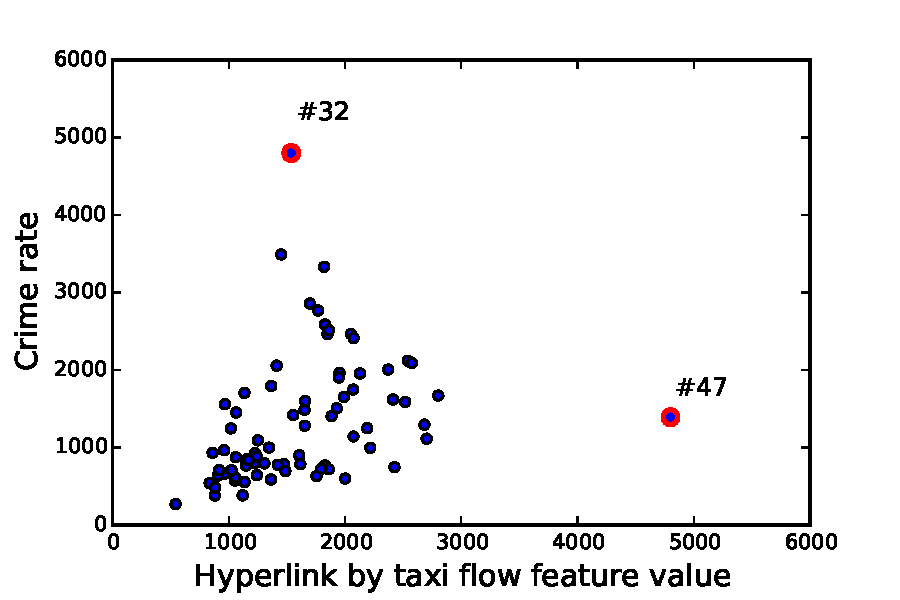
\includegraphics[width=0.8\textwidth]{fig/taxi-flow-percent.pdf}
\caption{Correlation between taxi flow feature and crime rate. In the plot, we marked out two outliers and their corresponding community area ID.}
\label{fig:taxi-corr}
\end{figure}



%%%%
\nop{
\begin{figure}[t]
\centering
\subfigure[Arts POI w.r.t. crime count]{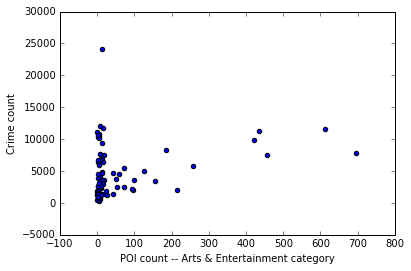
\includegraphics[width=0.23\textwidth]{fig/poi-arts.png}}
\subfigure[Arts POI w.r.t. crime rate]{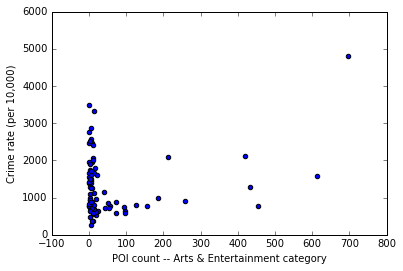
\includegraphics[width=0.23\textwidth]{fig/poi-arts-crimeRate.png}}
\caption{Comparison between the correlation of arts POI category count w.r.t. crime count and crime rate. The crime rate is crime count normalized per 10,000 population. \textred{draw fitted line, show $R^2$ error}}
\label{fig:demo-extra}
\end{figure}
}

\nop{
It is widely believed that the two geospatially close neighborhoods have higher interactions, and thus the crime rate is similar. 


In Table~\ref{tb:spatf}, the correlations between spatial flow and crime count are presented. Overall, the geographical influence is positively correlated with the crime count. At community area level, the geographical influence has a Pearson correlation coefficient of $0.4415$ with the actual crime count. In the crime prediction setting, the various communities have different areas and number of residents. In order to make fair comparison and eliminate the population effects, it is reasonable to compare the spatial flow against crime rate, namely the crime count per 10,000 population. In the second setting, we show the result of using crime rate, and there is a significant increase in the correlation.

At tract level, the spatial flow correlation with crime is reduced, as shown in the third and fourth row of Table~\ref{tb:spatf}. The reason is that tract is a relatively small geographical area, which is usually populated by $4,000$ people\footnote{Census Tract \url{http://www.census.gov/geo/reference/gtc/gtc_ct.html}}. The crimes are usually not commuted too close to the affenders' home.  

\begin{table}[h!]
\caption{Correlation between geographical neighbor feature and crime count.}
\label{tb:spatf}
\centering
\begin{tabular}{|l|r|}
\hline
Settings & correlation \\ \hline
CA level, crime count  & 0.4415 \\ \hline
CA level, crime rate per 10,000 population & 0.5969 \\ \hline
Tract level, crime count with social flow & 0.2377 \\ \hline
Tract level, crime rate per 10,000 population & 0.0771 \footnote{Census data is not 2010}\\ \hline
\end{tabular}
\end{table}



\begin{table}[h!]
\caption{Correlation between social flow and crime count.}
\label{tb:lehd}
\centering
\begin{tabular}{|l|r|}
\hline
Settings & correlation \\ \hline
CA level, crime count & 0.2072 \\ \hline
CA level, crime count, weighted social flow & 0.3217 \\ \hline
CA level, crime rate per 10,000 population & 0.5898 \\ \hline
CA level, crime rate, weighted social flow & 0.6014 \\ \hline
Tract level, crime count & 0.4462 \\ \hline
Tract level, crime rate per 10,000 population & 0.1306 \footnote{Census data is not 2010}\\ \hline
\end{tabular}
\end{table}



Table~\ref{tb:taxi} shows the correlation between taxi flow feature and crime. Under different settings, the taxi flow keep a positive correlation with the crime.


\begin{table}[h]
\caption{The correlation between taxi flow and crime}
\label{tb:taxi}
\begin{tabular}{|l|r|}
\hline
Settings & Correlation Coefficient \\\hline
Taxi flow count, crime rate & 0.2337 \\ \hline
Taxi flow count, crime count & 0.2514 \\ \hline
Taxi flow percentage, crime rate & 0.3315 \\ \hline
Taxi flow percentage, crime count & 0.3418 \\ \hline
\end{tabular}
\end{table}


}







% !TEX root = main.tex
\section{Experiments}
\label{ch5-sec:experiment}


\subsection{Settings}

We use four types of data as features, including demographics, POI, geographical influence, and taxi flow, to predict the total crime rates. The details of feature data are described in Section~\ref{ch2-sec:feature}, and a description of crime data is available in Section~\ref{ch5-sec:overview}. We conduct the crime prediction on five consecutive years, 2010 -- 2014. There are over 30 categories of crime, and many categories have sparse values over regions. Therefore, we only study the effect of crime categories in Section~\ref{sec:crime-cat}, and in the rest experiments, we predict the total crime rate.

The following four methods, e.g. regression kriging (RK), linear regression (LR), negative binomial regression (NB), and geographically weighted negative binomial regression (GWNBR), are evaluated. The regression kriging method employs a regression model to incorporate all features as auxiliary variables, and then applies kriging to estimate the regression residual. We add kriging as one of the baseline, mainly because kriging is one of the most widely used method for geospatial interpolation~\cite{OlWe90}.

We evaluate the estimation accuracy under various feature combinations. The bandwidth of Gaussian kernel $h$ used for GWNBR is tuned separately under different settings. Refer to Section~\ref{sec:parameter} for more details on parameter tuning.

We adopt leave-one-out evaluation to estimate the crime rate of one geographic region given all the information of all the other regions. When we construct the spatial/social lag variable for the training data, the effect of testing region is completely removed. For example, if region $y_t$ is the testing region, the remaining $\{y_i | \forall i \text{ s.t. } i \neq t\}$ become the training set. For any $y_i$ in the training set, its geographical influence feature and taxi flow feature are constructed only from $\{y_i | \forall i \text{ s.t. } i \neq t\}$.

In the evaluation, we estimate the crime rate for testing community areas. The accuracy of estimation is evaluated by mean absolute error (MAE) and mean relative error (MRE).

\begin{align}
MAE & = \frac{\sum_i |y_i - \hat{y_i}| }{n} \\
MRE & = \frac{\sum_i |y_i - \hat{y_i}|} {\sum_i y_i }
\end{align}



\begin{table}
\centering
\caption{Performance evaluation on total crime rate prediction. Various feature combinations are shown in each column. The linear regression model,  negative binomial model, and geographically weighted negative binomial model are compared by year group. }
\label{tb:perf}

\resizebox{!}{0.45\textheight}{
\begin{tabular}{|c|c|c|c|c|c|c|}
\hline
\multicolumn{3}{|c|}{} & \multicolumn{4}{|c|}{Settings} \\ \hline
\multicolumn{3}{|c|}{Column ID} & 1 & 2 & 3 & 4  \\ \hline
\multicolumn{2}{|c|}{\multirow{4}{*}{Features$^1$}}	& \textbf{D}emo &  \checkmark& \checkmark& \checkmark& \checkmark \\ \cline{3-7}
\multicolumn{2}{|c|}{}	& \textbf{G}eo & \checkmark & \checkmark& \checkmark& \checkmark \\ \cline{3-7}
\multicolumn{2}{|c|}{}	& \textbf{P}OI & &\checkmark & & \checkmark \\ \cline{3-7}
\multicolumn{2}{|c|}{}	& \textbf{T}axi & & & \checkmark& \checkmark \\ \hline
Year & Model$^2$ & Error & \multicolumn{4}{|c|}{} \\ \hline
                       &  & MAE & 463.68 & 461.67 & 452.39 & 421.59 \\ \cline{3-7}
                       & \multirow{-2}{*}{RK} & MRE & 0.346 & 0.344 & 0.337 & 0.314 \\ \hhline{|~|*{6}{-|}}
  \rowcolor{Gray}  
  \cellcolor{white} &  \cellcolor{white} & MAE &  394.78 & 432.45 & 413.80 & 404.00\\ \hhline{|~|~|*{5}{-|}}
  \rowcolor{Gray}
  \cellcolor{white} & \cellcolor{white}\multirow{-2}{*}{LR}& MRE &  0.295 & 0.323 & 0.309 & 0.301\\ \hhline{|~|*{6}{-|}}
	
                       &  & MAE &  402.82 & 343.55 & 404.49  & 315.28\\ \cline{3-7}
                       & \multirow{-2}{*}{NB}	& MRE  & 0.301 & 0.256 & 0.302 & 0.235 \\ \hhline{|~|*{6}{-|}}
  \rowcolor{Gray2}
  \cellcolor{white}	& \cellcolor{white} & MAE & 343.44 & 332.38 & 327.20 & \textbf{265.93}\\ \hhline{|~|~|*{5}{-|}}
  \rowcolor{Gray2}
  \cellcolor{white}\multirow{-8}{*}{2010} & \cellcolor{white}\multirow{-2}{*}{GWNBR} & MRE & 0.256 & 0.248 & 0.244 & \textbf{0.198} \\ \hline
	
                       &  & MAE & 460.83 & 422.01 & 424.05 & 430.77 \\ \cline{3-7}
                       & \multirow{-2}{*}{RK} & MRE & 0.358 & 0.328 & 0.330 & 0.335 \\ \hhline{|~|*{6}{-|}}
  \rowcolor{Gray}  
  \cellcolor{white} & \cellcolor{white} & MAE & 380.08 & 422.94 & 402.63 & 402.81\\  \hhline{|~|~|*{5}{-|}}
  \rowcolor{Gray}
  \cellcolor{white} & \cellcolor{white}\multirow{-2}{*}{LR}& MRE & 0.296 & 0.329 & 0.313 & 0.313\\ \hhline{|~|*{6}{-|}}
                       & & MAE & 391.26 & 340.49  & 396.59  & 325.34 \\ \cline{3-7}
                       & \multirow{-2}{*}{NB}	& MRE  & 0.304 & 0.265  & 0.308  & 0.253 \\ \hhline{|~|*{6}{-|}}
  \rowcolor{Gray2}
  \cellcolor{white}	& \cellcolor{white} & MAE & 330.04 & 325.56 & 322.77  & \textbf{275.61}\\ \hhline{|~|~|*{5}{-|}}
  \rowcolor{Gray2}
  \cellcolor{white}\multirow{-8}{*}{2011}	&\cellcolor{white}\multirow{-2}{*}{GWNBR}	& MRE  & 0.257 & 0.253 & 0.251 & \textbf{0.214} \\ \hline

                       & & MAE & 455.94 & 418.04 & 438.13 & 412.55 \\ \cline{3-7}
                       & \multirow{-2}{*}{RK} & MRE & 0.368 & 0.338 & 0.354 & 0.333 \\ \hhline{|~|*{6}{-|}}
  \rowcolor{Gray}
  \cellcolor{white} &  \cellcolor{white} & MAE & 375.62 & 423.88 & 402.69 & 404.06\\ \hhline{|~|~|*{5}{-|}}
  \rowcolor{Gray}
  \cellcolor{white} & \cellcolor{white}\multirow{-2}{*}{LR}& MRE & 0.304 & 0.343 & 0.325 & 0.327\\ \hhline{|~|*{6}{-|}}

                       & & MAE & 395.82 & 349.09 & 399.99 & 342.41  \\ \cline{3-7}
                       & \multirow{-2}{*}{NB}	& MRE  & 0.320 & 0.282  & 0.323  & 0.277  \\ \hhline{|~|*{6}{-|}}
		\rowcolor{Gray2}
		\cellcolor{white}	& \cellcolor{white} & MAE  & 332.70 & 342.95 & 334.83 & \textbf{330.51} \\ \hhline{|~|~|*{5}{-|}}
		\rowcolor{Gray2}
		\cellcolor{white}\multirow{-8}{*}{2012}	&\cellcolor{white}\multirow{-2}{*}{GWNBR}	& MRE  &0.269  & 0.277 & 0.270 & \textbf{0.267} \\ \hline
	
                       & & MAE & 408.90 & 468.39 & 457.20 & 413.77 \\ \cline{3-7}
                       & \multirow{-2}{*}{RK} & MRE & 0.360 & 0.412 & 0.402 & 0.363 \\ \hhline{|~|*{6}{-|}}
  \rowcolor{Gray}
  \cellcolor{white} & \cellcolor{white} & MAE & 369.24 & 433.48 & 387.58 & 400.75\\ \hhline{|~|~|*{5}{-|}}
  \rowcolor{Gray}
  \cellcolor{white} & \cellcolor{white}\multirow{-2}{*}{LR}& MRE & 0.325 & 0.381 & 0.341 & 0.352\\ \hhline{|~|*{6}{-|}}
                       &  & MAE & 390.09 & 348.16 & 389.79 & 324.94 \\ \cline{3-7}
                       & \multirow{-2}{*}{NB}	& MRE & 0.343 & 0.306  & 0.343  & 0.286 \\ \hhline{|~|*{6}{-|}}
  \rowcolor{Gray2}
  \cellcolor{white}	& \cellcolor{white} & MAE & 319.75 & 334.58  & 316.70 & \textbf{316.34}\\ \hhline{|~|~|*{5}{-|}}
  \rowcolor{Gray2}
  \cellcolor{white}\multirow{-8}{*}{2013}	&\cellcolor{white}\multirow{-2}{*}{GWNBR}	& MRE   & 0.281 & 0.294 & 0.279 & \textbf{0.278} \\ \hline
	
                       & & MAE & 404.76 & 365.14 & 453.07 & 380.83 \\ \cline{3-7}
                       & \multirow{-2}{*}{RK} & MRE & 0.398 & 0.359 & 0.446 & 0.374 \\ \hhline{|~|*{6}{-|}}
  \rowcolor{Gray}
  \cellcolor{white} & \cellcolor{white} & MAE & 329.93 & 386.9 & 355.83 & 358.47\\ \hhline{|~|~|*{5}{-|}}
  \rowcolor{Gray}
  \cellcolor{white} & \cellcolor{white}\multirow{-2}{*}{LR}& MRE &   0.325 & 0.381 & 0.35 & 0.353\\ \hhline{|~|*{6}{-|}}

                       &  & MAE & 347.39 & 303.59  & 348.71  & 289.52\\ \cline{3-7}
                       & \multirow{-2}{*}{NB} & MRE & 0.342  & 0.299  & 0.343  & 0.285 \\ \hhline{|~|*{6}{-|}}
  \rowcolor{Gray2}
  \cellcolor{white}	& \cellcolor{white} & MAE & 282.35  & 280.58  & 274.16  & \textbf{272.51}\\ \hhline{|~|~|*{5}{-|}}
  \rowcolor{Gray2}
  \cellcolor{white}\multirow{-8}{*}{2014}	&\cellcolor{white}\multirow{-2}{*}{GWNBR} & MRE & 0.277  & 0.276 & 0.270 & \textbf{0.268} \\ \hline
\end{tabular}
}

\footnotesize{$^1$ Demo -- demographic features, Geo -- geographical influence, POI -- POI features, Taxi -- taxi flow feature.}
\footnotesize{$^2$ RK -- Regression Kriging, LR -- Linear Regression, NB -- Negative Binomial Regression, GWNBR -- Geographically Weighted Negative Binomial Regression.}
\end{table}



\subsection{Performance on Different Feature Combinations}

The leave-one-out evaluation results are shown in Table~\ref{tb:perf}. Ideally, we should show all the possible combinations of feature groups, which will result in 15 combinations. Due to the space limit, we show 4 combinations in Table~\ref{tb:perf}. Setting 1 (\textbf{D+G}) represents the traditional features used in criminology literature. Setting 2 (\textbf{D+G+P}) and setting 3 (\textbf{D+G+T}) are used to examine the individual effects of new features on POI and Taxi flows. Setting 4 (\textbf{D+G+P+T}) studies the combined effects of all features.

\subsubsection{POI Feature} 
Adding POI features improves the accuracy of the NB model (see setting 2 vs. setting 1 and setting 4 vs. setting 3 in Table~\ref{tb:perf}). The POI distribution reflects the functionality of a region. The most correlated POI major category is ``professional'', under which there are a lot of venues like transportation center and conventional center. These are locations with more dynamic movements of people. Such location information is not reflected in any of other features. POI thus provides  unique information and it shows that using big data can benefit us in advancing the study of traditional crime inference problems. 

Another issue worth discussing is whether POI is a surrogate of population features from demographics. That is, a region with more POIs is a region with higher population. However, as we see from Table~\ref{tb:perf}, the NB model using POI feature in addition to the demographic and geographic features always outperforms the model without the POI feature. This is because population from demographics reflects the number of residents in that region, but POI reflects dynamics of population (e.g., people go to venues for food, entertainment, or travel). Therefore, the dynamic population in POI further complements the residential population in demographics.


\subsubsection{Taxi Flow} 
%The taxi flow is shown to improve the inference accuracy (see Table~\ref{tb:perf} for column 3 vs. column 1 and column 4 vs. column 2). This validates our hypothesis that crimes do not only correlate with nearby regions but also correlate through hyperlinks on the space (i.e., the taxi flow). 

To test our hypothesis that crimes do not only correlate with nearby regions but also correlate through hyperlinks on the space (i.e., the taxi flow), we examine if considering taxi flow improves the inference accuracy. Comparing setting 3 with setting 1 in Table~\ref{tb:perf}, we find that the improvement by taxi flow is not obvious for NB. However, comparing setting 4 with setting 2, we observe a much more significant accuracy boost. The reason could be that the taxi flow further complements the POI data. When POI information is missing from the predictor, the city dynamics captured by taxi flow are weakened as well.

Meanwhile, we note that incorporating the new urban data (POIs and taxi flow) significantly improves the performance of the NB model. Specifically, comparing  setting 4 with setting 1, the improvements in MRE are 6.6\%, 5.1\%, 4.3\%, 5.7\%, and 5.7\% for the five years, respectively.


\subsubsection{Feature Consistency}

In this section, we study the consistency of features as shown in Figure~\ref{fig:fcon}. We get the effect of adding POI feature by comparing setting 2 and setting 1 in Table~\ref{tb:perf}. Similarly, setting 3 vs setting 1 shows the effect of adding taxi, and setting 4 vs setting 1 shows the effect of adding both. For each method we show number of years in y-axis, in which the added feature improves the model performance.

We observe that adding both features shows the best performance for both NB and GWNBR, meanwhile it is not necessarily the best for other models. For example, LR shows that setting 1 is better than setting 4 over different years. RK shows that setting 1 is better than setting 4 in year 2013 but not other years. We argue that it is crucial to use the right model to captures extra information and achieves consistent results.

\begin{figure}[t]
\centering
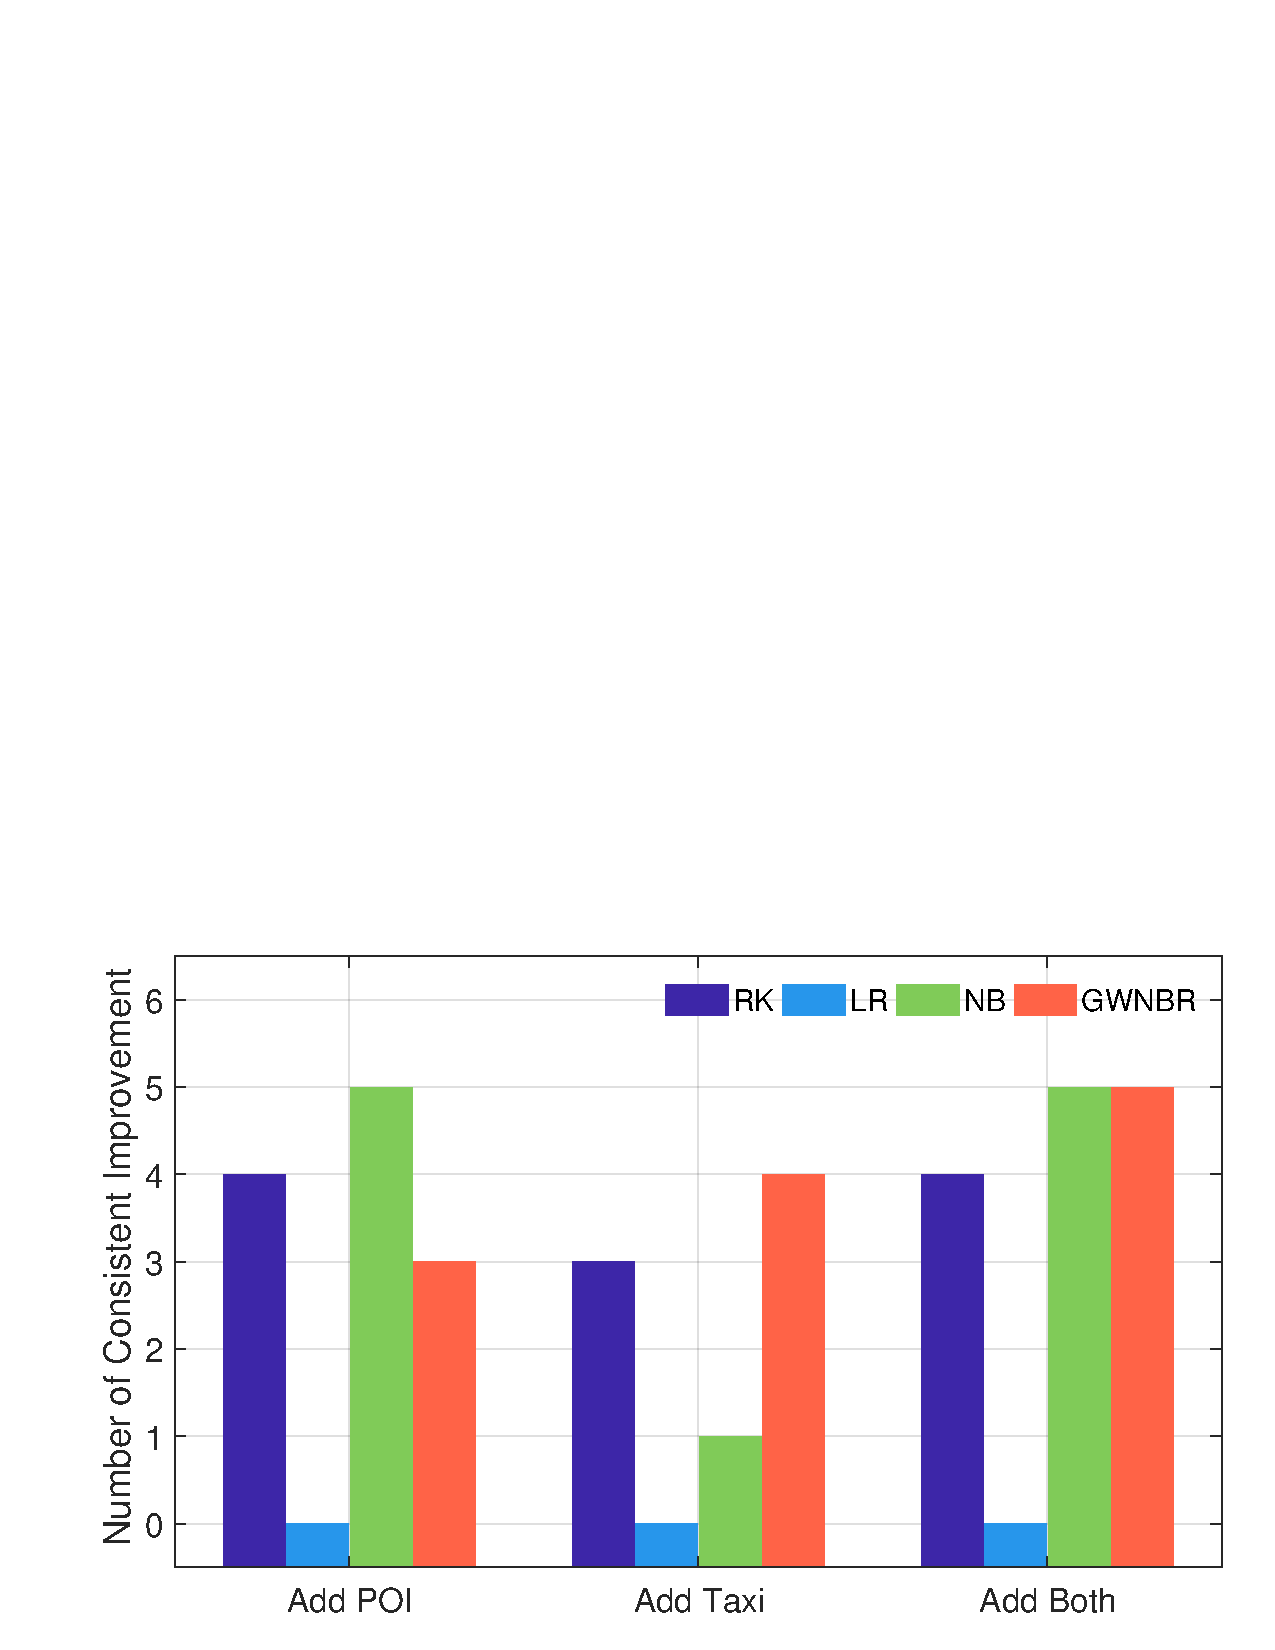
\includegraphics[width=0.7\linewidth]{fig/feature_consistency.pdf}
\caption{The feature consistency results. The x-axis shows the effect of adding different features. The y-axis shows number of years that shows improvement.}
\label{fig:fcon}
\vspace{-3mm}
\end{figure}




\subsection{Performance on Different Methods}

In this section, we compare the prediction error of different methods, and we have the following observations.

\subsubsection{Regression Kriging vs. Other Regressions}
We observe that kriging method usually performs worse than other regression methods. The reason is that the kriging method is designed for interpolation and the objective is to minimize the estimation variance. Kriging method usually overestimates a local minimum and underestimates a local maximum due to the fact the kriging uses average to interpolate. For the crime rate prediction problem, other regression methods directly optimize the prediction error, and therefore outperforms the kriging method.

\subsubsection{Negative Binomial Regression vs. Linear Regression}
In Table~\ref{tb:perf},  we can see that under most settings, the negative binomial regression significantly outperforms the linear regression (with only a few exceptions when using demographic features and geographic features). When using all the features, NB is significantly better than LR with at least $5\%$ improvement in MRE.
There are two reasons why the negative binomial regression is more appropriate for crime rate estimation than linear regression.
First, negative binomial regression guarantees the prediction variable is non-negative. Second, it is difficult to get very precise estimates of crime rate, and the negative binomial regression allows a large variance in the estimated crime rate. 


\subsubsection{GWNBR vs. NB, and the Effectiveness of Non-Stationary Model}
Next, we compare the negative binomial regression with the geographically weighed negative binomial regression. As shown in~Table~\ref{tb:perf}, the GWNBR model consistently outperforms the NB model in all experiment settings, which validate our hypothesis that the correlation among crime rate and other features are non-stationary. 

In addition, comparing setting 2 (\textbf{D+G+P}) or setting 3 (\textbf{D+G+T}) with setting 1 (\textbf{D+G}) in Table~\ref{tb:perf}, we observe that the performance improvement for GWNBR by POI feature or taxi flow separately is not obvious. However, when all features (\textbf{D+G+P+T}) are used, GWNBR consistently gives lower estimation error than using the traditional features only (\textbf{D+G}). In the best case (years 2010 and 2011), GWNBR reduces the MAE by over 15\%. This again suggests that the POI feature and taxi flow complement each other, and that incorporating both features yields the best inference accuracy.


In view of the superior performance of GWNBR, in all the following experiments we only refer to the performance of GWNBR.


\subsection{Parameter Sensitivity}
\label{sec:parameter}

In the GWNBR model, the bandwidth parameter $h$ in Equation~(\ref{eq:gwr-gkn}) controls the influence of a nearby training sample. There are several approaches to determine the bandwidth $h$~\cite{WLL+15}. Here, we adopt the cross validation approach to estimate a best $h$ from data. More specifically, we fit a model on the training data and report the prediction error on the testing data. The best $h$ should lead to the lowest prediction error.


In this experiment, we use data from year 2010 to study the effect the bandwidth $h$ on the performance of GWNBR. Using a data-driven approach, we adopt the mean absolute error as a measure of fit. In Figure~\ref{fig:gwnbr-h}, we plot the MAE against bandwidth under leave-one-out setting. It is clear that the optimal bandwidth is $5.8$, which gives us the lowest MAE. Furthermore, we observe that when $h$ becomes larger, the performance of GWNBR model approaches to the NB model (with a MAE of $310$). This observation is consistent with the model, because an infinitely large bandwidth gives all samples the same weight, which makes the GWNBR essentially  an NB model. 

\begin{figure}[h]
	\centering
	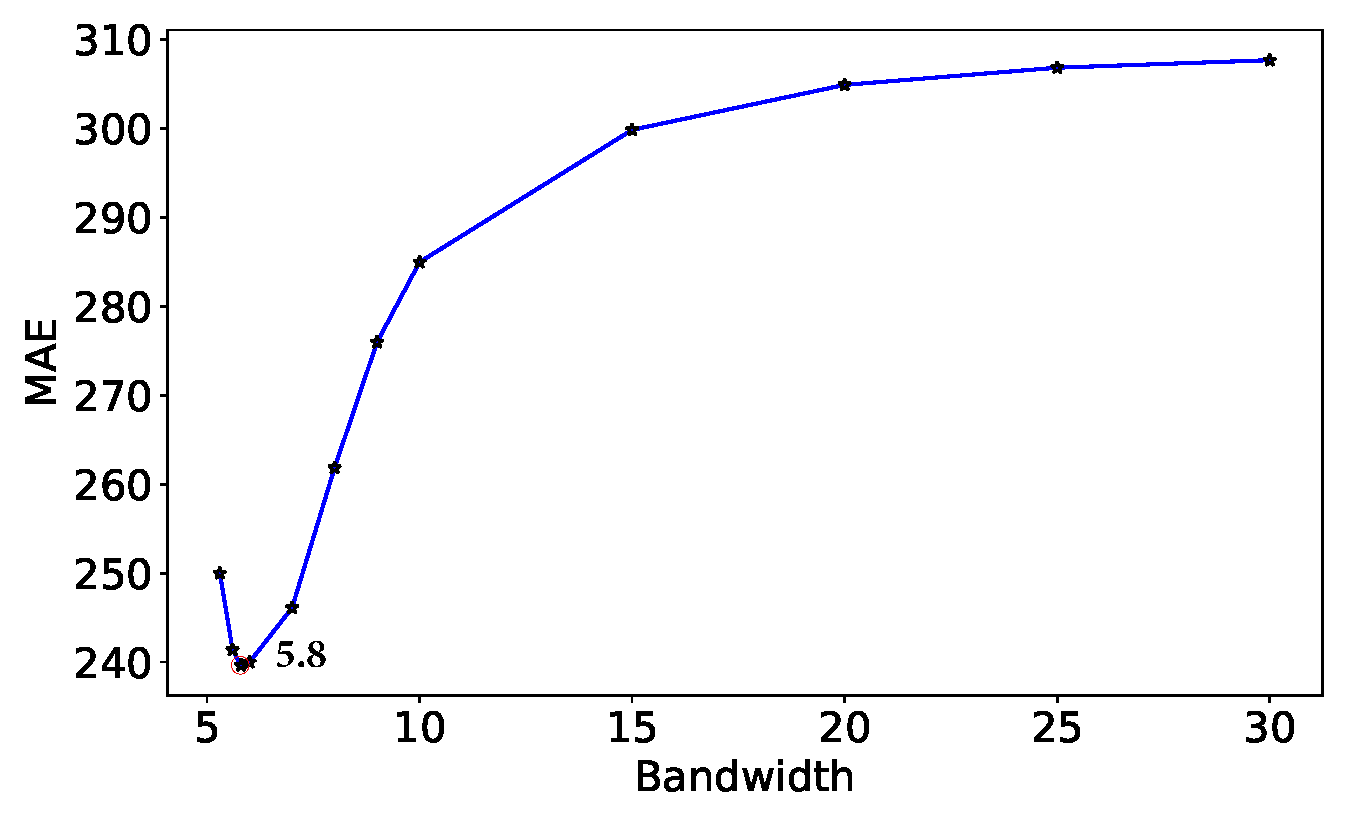
\includegraphics[width=0.7\linewidth]{fig/para_sensitive.pdf}
	\caption{Bandwidth sensitivity analysis for geographically weighted negative binomial regression.}
	\label{fig:gwnbr-h}
\vspace{-3mm}
\end{figure}




%\medskip
%\noindent \textbf{Taxi Flow normalization.} 
\nop{
\subsubsection{Taxi Flow Normalization}
The taxi flow represents the interactions among community areas. There are several different approaches to incorporate the taxi flow into the model.  First, we can use the raw taxi count as a weight on crime from other neighborhoods. One issue with the raw count is the concentration of taxi trips distribution in the downtown area. Consider the following example. In the downtown area, the average taxi flow count is \num{1000} between any pair of community areas, while the average of suburbs is $100$. When we propagate crime by raw taxi count, the same amount of crime in downtown is propagated with a  $10$ times higher coefficient than that of suburb. 


To address this issue, we can normalize the taxi flow, and there are two different approaches to normalize. 1) We can normalize the taxi flow by the total incoming traffic of the destination community area, and the semantics of this normalization is splitting the crime in the destination to all its neighbors. 2) Alternatively, we can normalize the taxi flow by the outgoing total trips in the source community area. This normalization assumes the crime in each source community is spread out by the flow.  The two normalization methods are shown in Figure~\ref{fig:taxiflow-norm}.


\begin{figure}[h]
\centering
\begin{tikzpicture}
\node[right]  at (0,0) {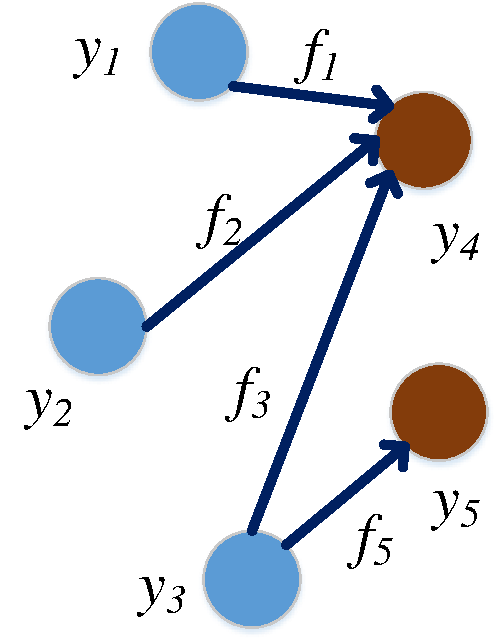
\includegraphics[width=0.12\textwidth]{fig/taxiflow-normalization.pdf}};
\node[align=left, above right] at (2.3, 0.3) {Normalization by source: \\ $F^t_4 = \frac{f_1}{f_1} y_1 + \frac{f_2}{f_2} y_2 + \frac{f_3}{f_3+f_5} y_3$};
\node[align=left, below right] at (2.3, -0.3) {Normalization by destination:  \\ $F^t_4 = \frac{f_1}{f_1+f_2+f_3} y_1 + \frac{f_2}{f_1+f_2+f_3} y_2 + \frac{f_3}{f_1+f_2+f_3} y_3$};
\end{tikzpicture}
\caption{Two different normalization schemes.}
\label{fig:taxiflow-norm}
\end{figure}



\begin{table}[h]
\centering
\caption{Various approaches to construct taxi flow feature. Estimation for crime in 2013 with all other features.}{
\label{tb:tf-design}
\begin{tabular}{|l|c|c|}
\hline
\multirow{2}{*}{Settings} & \multicolumn{2}{|c|}{GWNBR} \\ \cline{2-3}
	& MAE & MRE \\ \hline
Taxi flow count & 364.02 & 0.320 \\ \hline
Taxi flow normalized by source & 324.15 & 0.285 \\ \hline
Taxi flow normalized by destination & 304.26& 0.268\\ \hline
\end{tabular}}
\end{table}


In Table~\ref{tb:tf-design} we compare the different approaches to handle the taxi flow. Using raw taxi flow count is clearly not a good option, due to the unbalanced data distribution. We also observe that normalizing taxi flow by destination is better than normalization by source. The reason could be explained by the example given in Figure~\ref{fig:taxiflow-norm}. Suppose the focal region is a transportation hub, which has a lot of isolated regions connected to it. If we normalize the crime by source region, then the taxi flow feature of focal region is overestimated, since the coefficients of its neighbors do not sum to one. 
}



\subsection{Feature Importance}

In this section, we study the importance of features through significance tests.


From previous results, we see that combining POI features and taxi flow will help improve the estimation accuracy. Now we try to measure the significance of this accuracy boost by permutation tests. If a feature correlates with crime, when we randomly permute the values of this feature among neighborhoods, we will expect a higher error in crime rate estimation. So in each round of permutation, we can get an error in estimation. We compare the error with the original feature to the error distribution obtained from permutations. We conduct 1,000 rounds of permutations to approximately estimate the error distribution. The position of the original error in this distribution indicates the significance of this feature. For example, if the original error is smaller than 99\% of the errors from the permutations, the p-value is 0.01. 

\nop{
The permutation test procedure is described as follows. Each feature is randomly permuted for $1,000$ times. After each permutation, the leave one out evaluation is applied to get the accuracy measure (MAE, MRE). The $1,000$ rounds leave-one-out give us the distribution of accuracy measure under the null hypothesis that the permuted feature is irrelevant to the crime. We further calculate the probability that under the null hypothesis the error is smaller than the error in Table~\ref{tb:perf}, and this probability is our p-value.  }


\begin{table}
\centering
\caption{Estimated p-value for each feature. The p-value is defined as the possibility that a smaller error measure is observed under the null hypothesis. Permutation test is conducted on 2014 data with all features (D+G+P+T) used.}
\label{tb:permt}
\begin{tabular}{|c|c|c|c|c|c|c|}
\hline
\multirow{3}{*}{\makecell{Settings: \\D+G+P+T}} & \multicolumn{2}{c}{LR} & \multicolumn{2}{|c|}{NB} & \multicolumn{2}{|c|}{GWNBR}\\ \cline{2-7}
	& MAE & MRE & MAE & MRE & MAE & MRE \\ \cline{2-7}
	& 358.47 & 0.353 & 289.52 & 0.285 & 272.51 & 0.268\\ \hline
Feature & \multicolumn{6}{c|}{p-value} \\ \hline
D & 0.000 & 0.000 & 0.000 & 0.000 & 0.000 & 0.000\\ \hline 
G & 0.001 & 0.001 & 0.005 & 0.005 & 0.004 & 0.004  \\ \hline
P & 0.022 & 0.021 & 0.005 & 0.005 & 0.006 & 0.007\\ \hline
T & 0.000 & 0.000 & 0.080 & 0.079 & 0.049 & 0.052\\ \hline
\end{tabular}
\vspace{-3mm}
\end{table}


In Table~\ref{tb:permt}, the p-values of different features are reported. The demographics feature is the most significant feature with estimated p-value being $0.00$. In all the $1,000$ random permutations of demographic feature, we never observe an error lower than the original error.  The proposed POI distribution and taxi flow are significant as well, with  p-values of $0.6\%$ and $4.9\%$ for the GWNBR.  We notice that the taxi flow has a p-value around $5\%$ instead of close to $0$. One reason is that the taxi flow overlaps with geographic feature. Thus, permuting taxi flow may not have a critical influence on the estimation error in certain cases.

%\footnotetext{The taxi flow feature significance is not exactly the same as KDD paper, because we updated the taxi flow within a different time period. The observations on taxi flow are consistent with KDD. The geographic feature differs a lot from KDD paper. In KDD paper, we report geographic feature  not significant (with a p-value of $0.6$. This is due to an error in KDD submission. Here we correct this error, and geographic feature is significant with a p-value of $0.005$.}


\nop{
\subsubsection{Coefficient Study}

In our regression model, the coefficient also indicates the importance of features. We normalize the values of all features to the range $[0,1]$, so that coefficients are comparable. Note that, under the GWNBR setting, there are multiple models in one year. Therefore, we further compute the average coefficient of all the models within the same year. This average coefficient is meaningful, because all the models are trained on the same data samples with different weights. In Eq.~(\ref{eq:gwr-general}), the weight $\gamma_{ij}$ is applied on the error term, thus does not change the importance of any specific feature.  The top-6 features with the most significant coefficients are shown in Table~\ref{tb:fea-stability}. The top three rows in Table~\ref{tb:fea-stability} are features with positive coefficients, which implies positive correlations with the crime rate. The bottom three features are negatively correlated with the crime rate.

By comparing the coefficients over different years, we observe that the coefficients are relatively stable with respect to time. The most important feature is percentage black, which captures the demographics of residents. The other two important features are POI outdoors and POI food. We also find three POI categories are among the top negatively correlated features. They are shop, residence, and education categories. The reason is probably that 1) at those places the population is relatively stable such as residence, which provides less opportunity for crime; 2) those places have taken precautions against crime, such as shop.
 

\begin{table}[h]
\centering
\caption{The coefficients of the top-6 features over different years. There are 21 different features in total. We only show the top-3 features with the highest positive/negative coefficients, respectively.}
\label{tb:fea-stability}
\scalebox{0.9}{
	\begin{tabular}{|c|c|c|c|c|c|}
	\hline
	\multirow{2}{*}{Feature} & \multicolumn{5}{c|}{Year} \\ \cline{2-6}
		& 2010 & 2011 & 2012 & 2013 & 2014 \\ \hline \hline
	Percentage black & 0.662 & 0.698 & 0.762 & 0.724 & 0.532             \\ \hline
	POI outdoors recreation & 0.617 & 0.641 & 0.607 & 0.564 &0.850       \\ \hline
	POI food & 0.423 & 0.531 & 0.547 & 0.499 & 0.484   \\ \hline \hline
	POI education &-0.269 &-0.307 &-0.369 &-0.393 &-0.360   \\ \hline
	POI residence & -0.188 &-0.328 &-0.364 &-0.285 &-0.366   \\ \hline
	POI shops &-0.397 &-0.478 &-0.520 &-0.446 &-0.515        \\ \hline
	\end{tabular}
}
\end{table}
}


\subsection{Improvements in Different Regions}

The POI distributions and taxi flow patterns are different from region to region. It is interesting to find out whether they have a consistently positive impact in crime rate estimation. For POI feature, we calculate the difference in estimation error (MAE) between two setting 3 (D+G+T) and setting 4 (D+G+P+T). Similarly, the MAE difference between setting 2 and setting 4 is calculated for the taxi flow feature. The results are shown in Figure~\ref{fig:feat-area}.  A positive difference (blue area) indicates that adding the new feature helps reduce the estimation error, while a negative difference (red area) indicates that the new feature adds more noise to the data.  

\begin{figure}[h!]
\centering
\subfigure[POI]{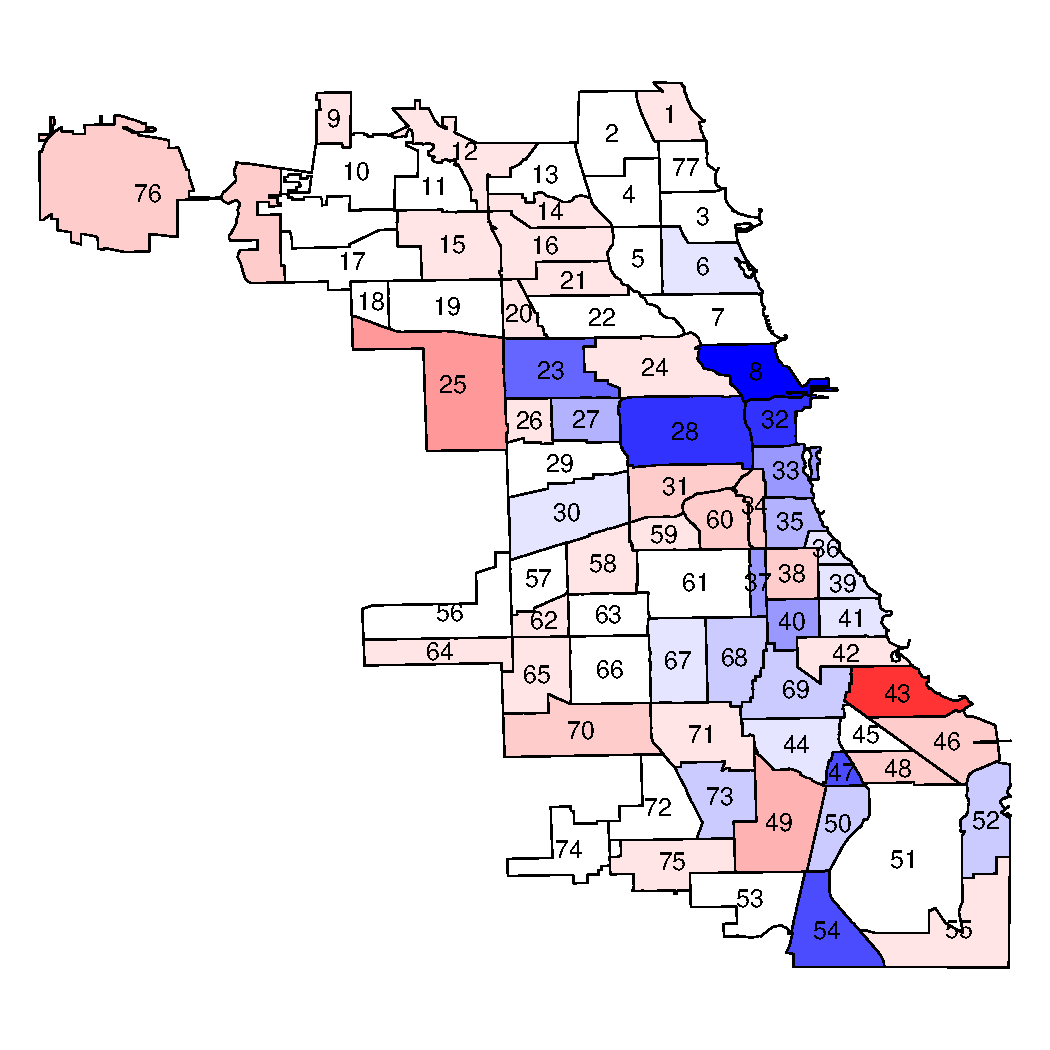
\includegraphics[width=0.45\linewidth]{fig/poi-improve_2014_new.pdf}}
\subfigure[Taxi flow]{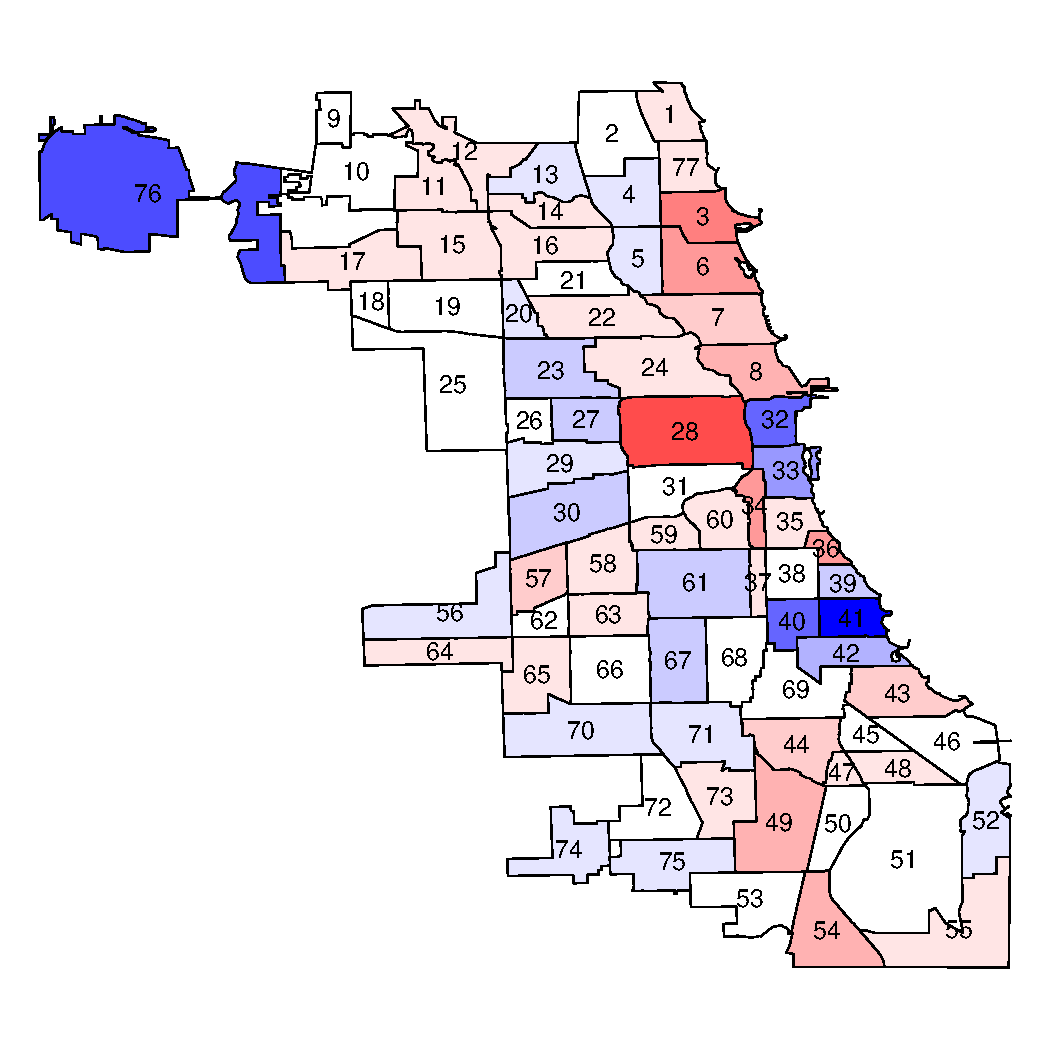
\includegraphics[width=0.45\linewidth]{fig/taxi-improve_2014_new.pdf}}
\caption{Performance improvement per region in year 2014. \textbf{Left:} The MAE difference of setting 3 and 4. \textbf{Right} The MAE difference of setting 2 and 4. The color blue means the MAE is reduced by adding the corresponding feature, while color red means the MAE is increased. The color saturation indicates the value of difference.}
\label{fig:feat-area}
\end{figure}


It is interesting to observe that in the downtown area, i.e. community areas \#8, \#32, and \#28, POI significantly improves the estimation accuracy. The reason is two fold. 1) The demographics information from census is mostly about the residing population in the focal area.  However, in the downtown area there are a lot of floating population groups conducting various social activities, and this is not reflected by the census demographics. The POI information, on the other hand, reflects the functionality of a region, hence complements the demographic information. 2) In the downtown area, there are more POIs than other places, which provide more complete information about the community profile.

As for the taxi flow feature, it helps the most in those suburb area, because the taxi flow reflects the social interaction in those areas. In the downtown area \#28 and \#8, the taxi flow feature incurs a relatively large estimation error. The reason is that the taxi flow distribution in Chicago is extremely skewed. Roughly 61\% of the Chicago taxi trips have a destination in the downtown area, which may result in the model over-propagating crime estimates from all of Chicago into the downtown area.




\section{Related Work}
\label{sec:related-work}


\textbf{Urban Data Heterogeneity.} Various urban data exhibit high degrees of correlation. As we collect more types of new urban data, we are able to solve a wide spectrum of urban problems. For example, a real-time air quality inference system is proposed in \cite{zheng2013u}, which uses not only historical air quality data, but also traffic flows, structure of roads, and POIs. Zheng et. al.~\cite{zheng2014diagnosing} diagnose New York City noise pollution with complaint records, road networks, and human check-ins. Real estate values are predictable given online user reviews~\cite{fu2014sparse} and offline human mobility data~\cite{wang:region}. Wang et. al.~\cite{wang2016crime, wang2017non} improve crime prediction accuracy by combining POI data and taxi flow data.

These existing works focus on mining the subtle correlations across different domains of data. We generalize the urban problems above as a learning task ,$f$, which maps some urban features to a target variable of interest. In this paper, we use crime prediction and average house price prediction as two examples. We study how to define the domain of urban problem, $f$, because only when $f$ is defined over a proper unit of study (e.g. community areas), the learned correlation is consistent and significant. \\

\noindent\textbf{Traditional Region Partition Methods.} Our problem falls into the region segmentation category. There are four main types of region partition methods that are widely used in the urban computing literature. First, a fixed sized grid is the most straightforward partition for travel time prediction~\cite{wang2016simple}, interpret traffic dynamics~\cite{wu2016interpreting}, and air quality inference~\cite{zheng2013u}. Second, existing administrative boundaries are also used for crime prediction~\cite{wang2016crime}. Third, clustering of point-wise urban data to get regions. For example, Li et. al.~\cite{li2015traffic} study the bike-sharing system and propose to estimate the supply/demand of bikes in a station cluster. Finally, other partitions are specifically designed for special needs. For example, Yuan et. al.~\cite{yuan2012discovering} employ the major road networks to partition a city into regions and learn the function of each region. Xu et. al.~\cite{xu2017understanding} partition a city by cellular tower coverages to study the mobile traffic pattern in urban environment. Zheng et. al.~\cite{zheng2015forecasting} use fan-shaped partitions to predict fine-grained air quality, because wind direction is an important indicator.


While various partition methods are used in existing urban problems, none of the partition methods explicitly take the learning task $f$ into consideration. It is worthy mentioning that most existing partition methods are purely based on cartographic information, and do not make use of the urban data properties. In this paper, we try to partition the city with an explicit objective. \\


\noindent\textbf{Discrete Optimizations.} The objective of our problem is a discrete optimization problem and is easy to derive. However, since the problem is NP-complete, it is challenging to efficiently find an optimal solution. MCMC sampling has been shown to be effective in optimizing discrete structures~\cite{strens2003evolutionary}. We follow this line of work and propose to use MCMC sampling to search for the optimal partition. During the MCMC sampling process, a lot of partitions are sampled but do not achieve better prediction results. To solve this issue, we follow the learning to optimize technique~\cite{li2016learning}, and propose to employ the reinforcement learning framework to learn where to sample the next partition that is most likely to improve the learning task, $f$.
\section{Conclusion}
\label{ch4-sec:conclusion}


In this chapter, we proposed a new problem called task-specific region partition. The problem is motivated by the fact that existing administrative boundaries are static regardless of the target variable, and we observed cases where it is necessary to have different partitions for different tasks. The task-specific region partition problem is NP-hard, and hence directly searching for a global optimal is difficult. Three variants of MCMC methods are proposed to solve this combinatorial optimization problem. First, a Naive MCMC that generates the next sample by random sampling. Second, a heuristic-based, Guided MCMC method that prefers to select from community areas with larger errors to generate the next sample. Finally, we employ reinforcement learning to automatically learn a sample strategy. Our methods are evaluated on two prediction tasks, i.e. crime prediction and real estate price prediction. The learned predictions consistently outperform the administrative boundaries in both tasks.